%\setcounter{secnumdepth}{+2}
\chapter{Implementação do Jogo}
%\chapter{Design and Development}
\label{cap4}

\section{Ferramentas e Tecnologias Utilizadas}

Várias ferramentas e diferentes tecnologias, foram utilizadas durante todo o processo de
desenvolvimento deste projeto, permitindo assim o seu desenvolvimento e facilitando a usa
implementação. Considerando ferramentas de construção de conteúdo digital até linguagens de programação.
Posto isto, as ferramentas e tecnologias utilizadas foram:

\begin{itemize}
    \item \textbf{\textcite{Blender}}: \textit{Software} de modelação 3D. Este \textit{software} foi utilizado para a modelação completa do cenário, assim como para a realização de ajuste no personagem (Criação de textura);
    \item \textbf{\textcite{Unity}}: \textit{Game Engine}, \textit{software} principal para o desenvolvimento do projeto. Ele é responsável pela junção dos \textit{asset's} com o código. Permitindo assim a construção de um experiência interativa. Além de ser utilizado para a criação de \textit{shaders}, que influenciam na construção visual do projeto;
    \item \textbf{Chat 3D:} Ferramenta de \ac{IA}. Utiliza para desenvolver o modelo 3D do personagem do jogo utilizando imagens 2D como base para a sua criação;
    \item \textbf{Gemini (Nano banana):} Ferramenta de \ac{IA}, utilizada para desenvolver o conceito do personagem, assim como utilizada para a criação de imagens ilustrativas do mesmo, que foram utilizadas no Chat 3D;
    \item \textbf{Processing:} \textit{Framework} de Java, que permite a a criação de imagens 2D. Esta tecnologia foi utilizada para a criação de algumas das partículas 2D presentes na \ac{UI}.;
    \item \textbf{Gimp e Affinity:} Ferramentas de edição de imagem. Foram utilizadas principalmente para ajustar as imagens geradas pelo Gemini;
    \item \textbf{C\#:} Linguagem de programação principal. É utilizada para a construção completa do jogo dentro da Unity. Responsável pela lógica do jogo, assim como implementação de sistema de \textit{gameplay};
    \item \textbf{Java:} Linguagem de programação utilizada no \textit{framework} Processing. Utilizada para a construção de certos \textit{assets} 2D;
\end{itemize}

\newpage

\section{Engenharia de Software}

\subsection{Diagrama de sistema de jogo}
\label{Sec:DiagramaSistemaJogo}

\begin{figure}[H]
    \centering
    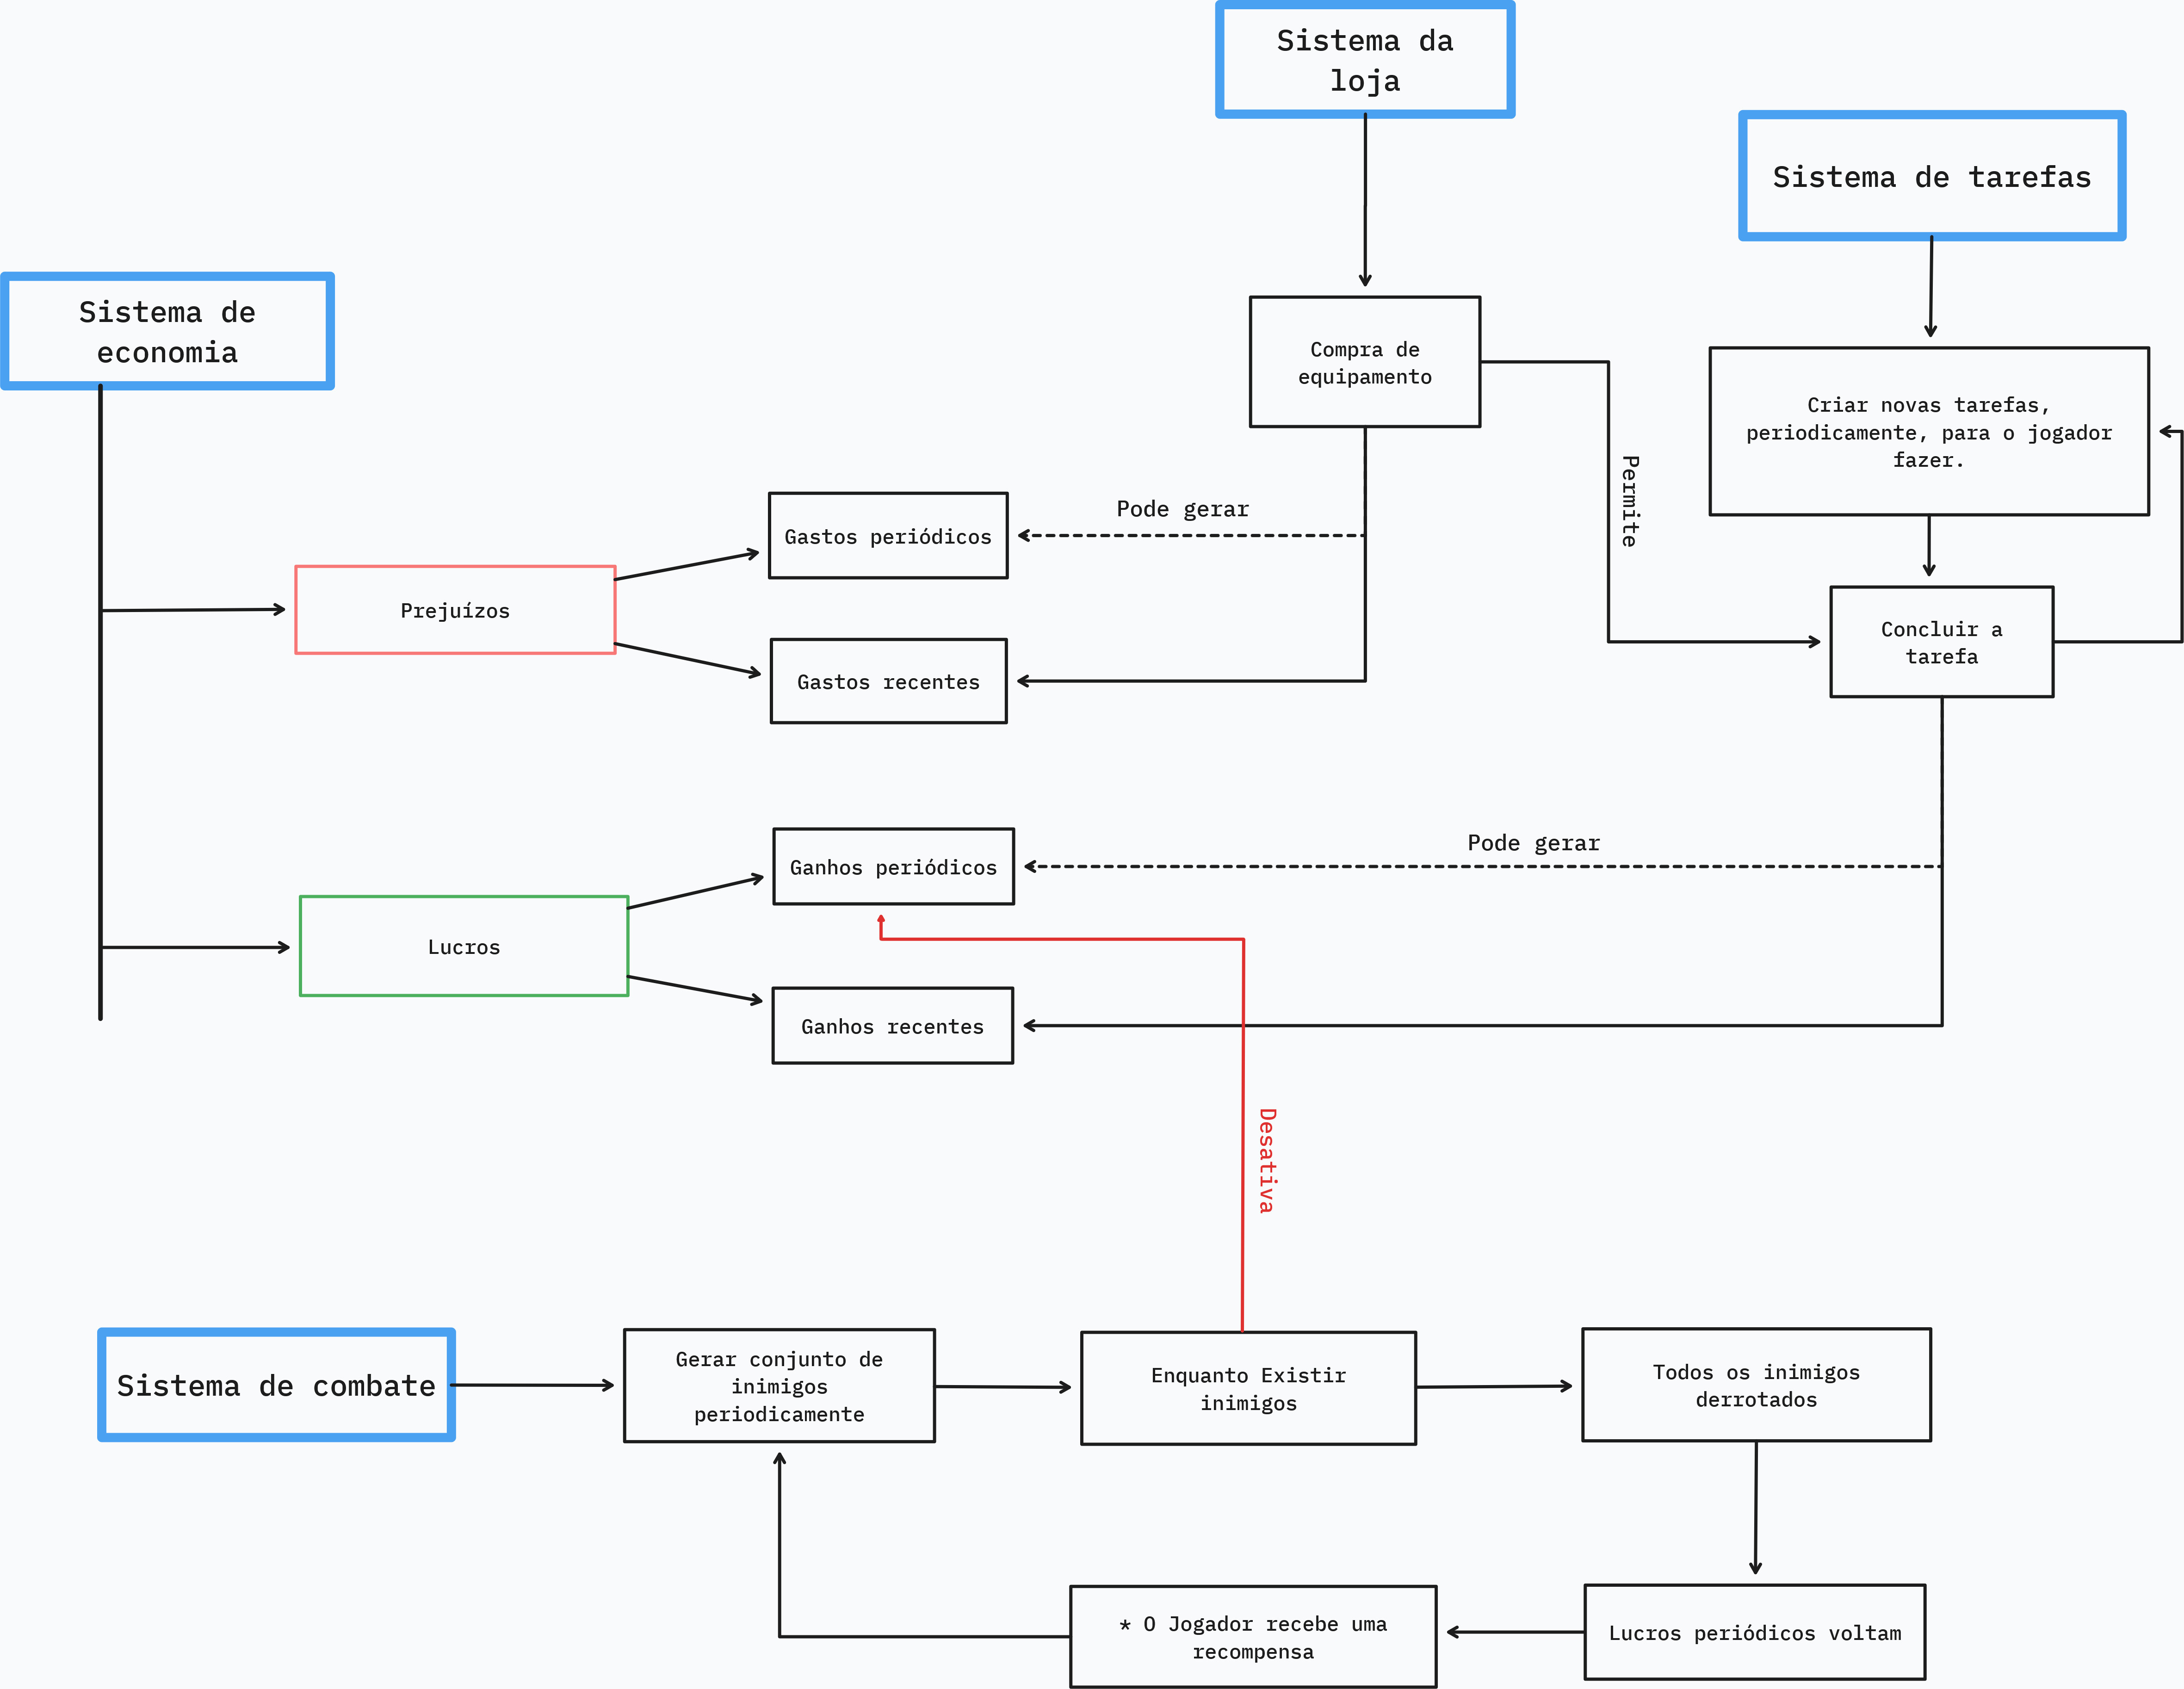
\includegraphics[width=1\textwidth]{Diagramas/diagrama_game.jpg}
    \caption{Diagrama de sistema do jogo.}
    \label{Diagrama_Sistema_Jogo}
\end{figure}

A Figura \ref{Diagrama_Sistema_Jogo} apresenta o diagrama de sistema do jogo, onde é possível observar os vários sistemas que compõem o jogo, assim como a interação entre eles.
Como é observável, todos os sistemas interagem com o sistema de economia, uma vez que esse sistema está fortemente ligado com a condição de derrota.
Além disso, é observável que o único sistema que permite com que o jogador ganhe dinheiro é o sistema de tarefas, o que faz com que seja através dele que o jogador consiga progredir no jogo, e como tal é o sistema que o jogador interage mais durante o jogo.

No diagrama, é possível observar que no sistema de combate, existe uma recompensa para o jogador.

\newpage

\subsection{Diagramas de caso de uso}
Diagramas de caso de uso, descrevem a funcionalidade de um sistema através da interação entre atores (utilizadores/sistema).
No contexto deste projeto os utilizadores são os jogadores e o sistema são os vários sistemas que compõem o jogo.
Nas subsecções subsequentes serão apresentados os diagramas de caso de uso dos três principais sistemas:
Tarefas, Loja e combate.

\subsubsection{Tarefas}

\begin{figure}[H]
    \centering
    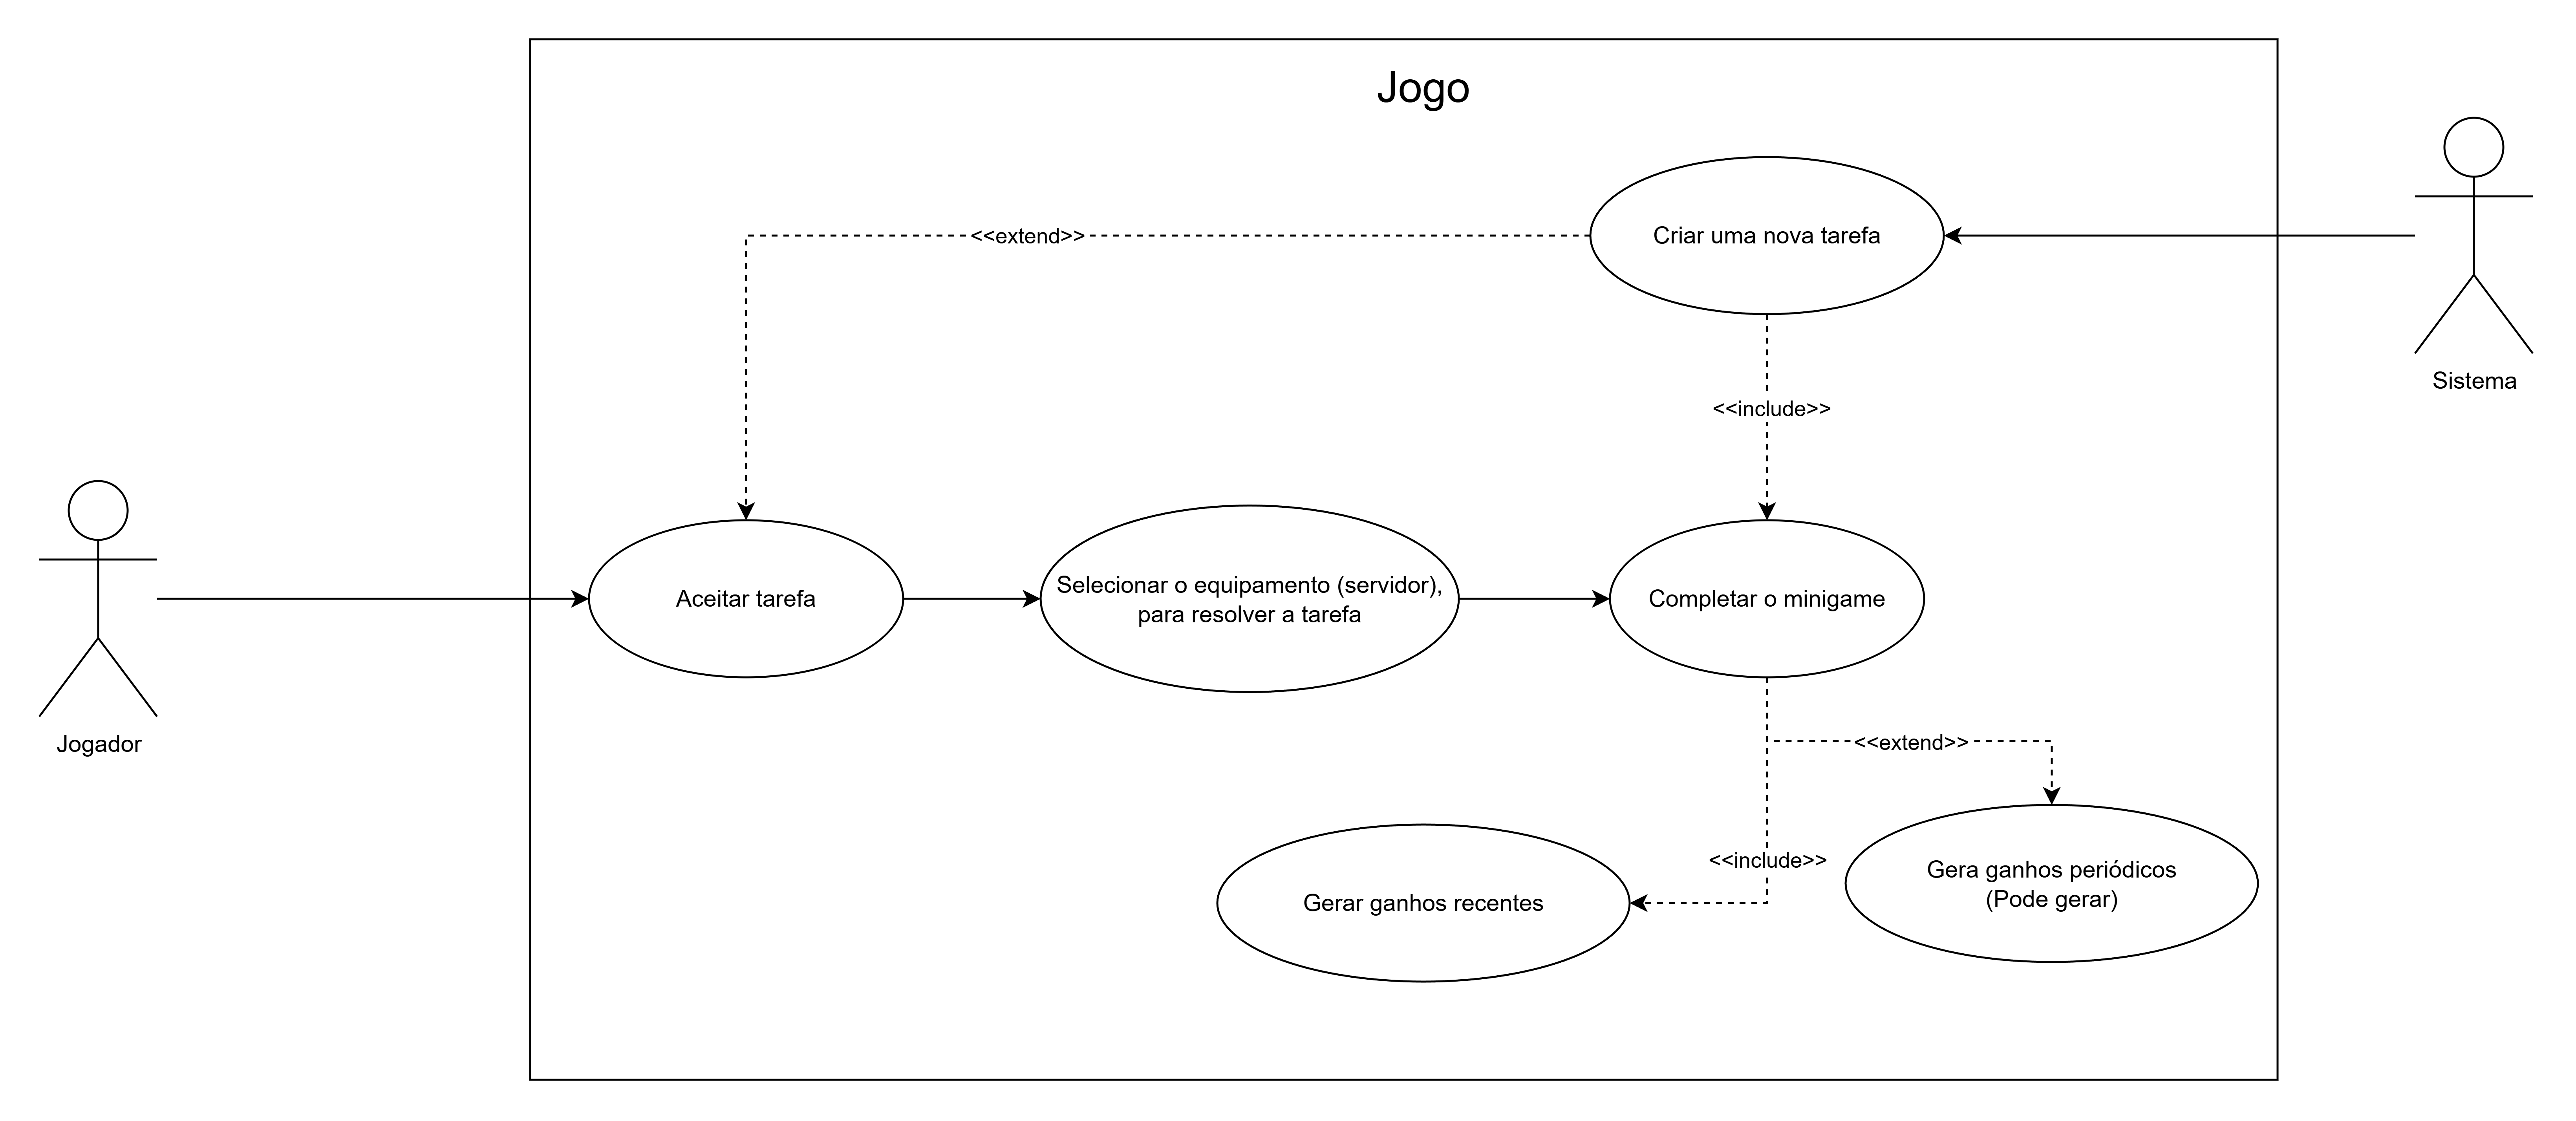
\includegraphics[width=0.9\textwidth]{Diagramas/Use_case_Tarefa.png}
    \caption{Diagrama de Caso de uso - Tarefas}
    \label{User_Case_Quests}
\end{figure}

O diagrama da Figura \ref{User_Case_Quests}, retrata a interação entre o jogador e o sistema de tarefas que periodicamente
cria tarefas para o jogador fazer, as quais, o jogador pode aceitar ou recusar. Uma vez que, cada tarefa
exigi recursos, o jogador pode escolhe recusar uma vez que pode não os ter ou acreditar que não compensa.

Além disso, assim como mostra o diagrama, 
ou concluir cada tarefa o jogador recebe uma certa quantidade de dinheiro,
podendo em certos casos receber outra quantidade de dinheiro de forma periódica.

\subsubsection{Loja}

\begin{figure}[H]
    \centering
    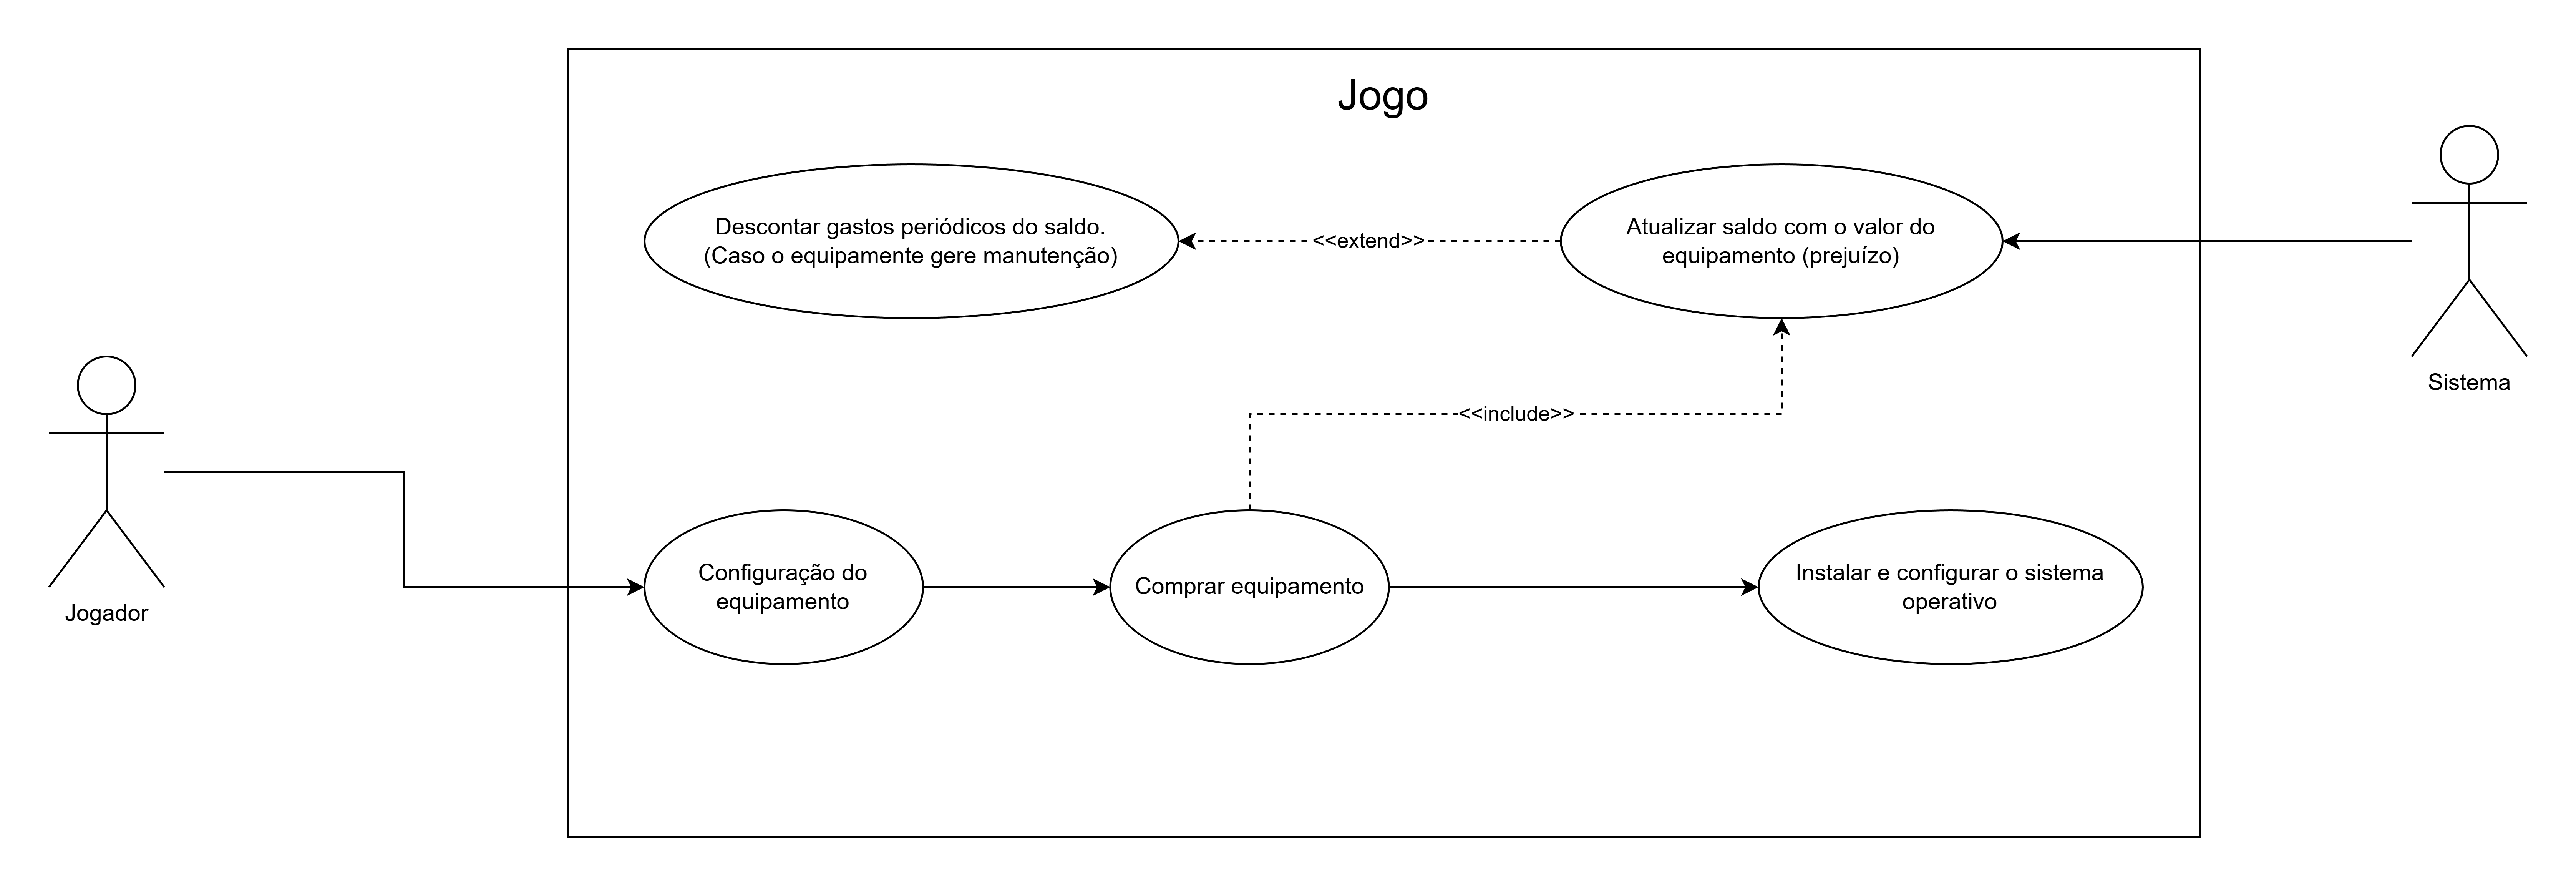
\includegraphics[width=0.9\textwidth]{Diagramas/Use_case_Shop.png}
    \caption{Diagrama de Caso de uso - Loja}
    \label{User_Case_Shop}
\end{figure}

A Figura \ref{User_Case_Shop} ilustra como o jogador interage com o sistema de Loja.
Os pontos mais relevantes das funcionalidades apresentadas são:
\begin{itemize}
    \item \textbf{Configuração de equipamento:} Uma vez que nesta etapa o jogador pode montar o servidor com o equipamento que quiser, dando assim liberdade para que o jogador possa ser criativo e conseguia balancear aspetos relevantes (como performance, armazenamento, refrigeração) face ao custo envolvido.
    \item \textbf{Instalação de sistema operativo:} É um passo à posterior a configuração do equipamento, onde o jogador tem que faz uma simulação de instalação de um sistema operativo, onde pode escolher o nome daquele servidor assim como a \textit{password}. Este passo é importante para a construção da experiência, uma vez que é um processo que acontece na realidade, e que tem um certo grau de complexidade, o que pode ajudar a construir uma experiência mais imersiva. Além disso, o nome atribuído ao servidor, é utilizado posteriormente para o jogador conseguir identificar o seu servidor, uma vez que o jogador pode ter mais do que um servidor.
\end{itemize}

\subsubsection{Combate}
\label{Sec:SistemaCombate}

\begin{figure}[H]
    \centering
    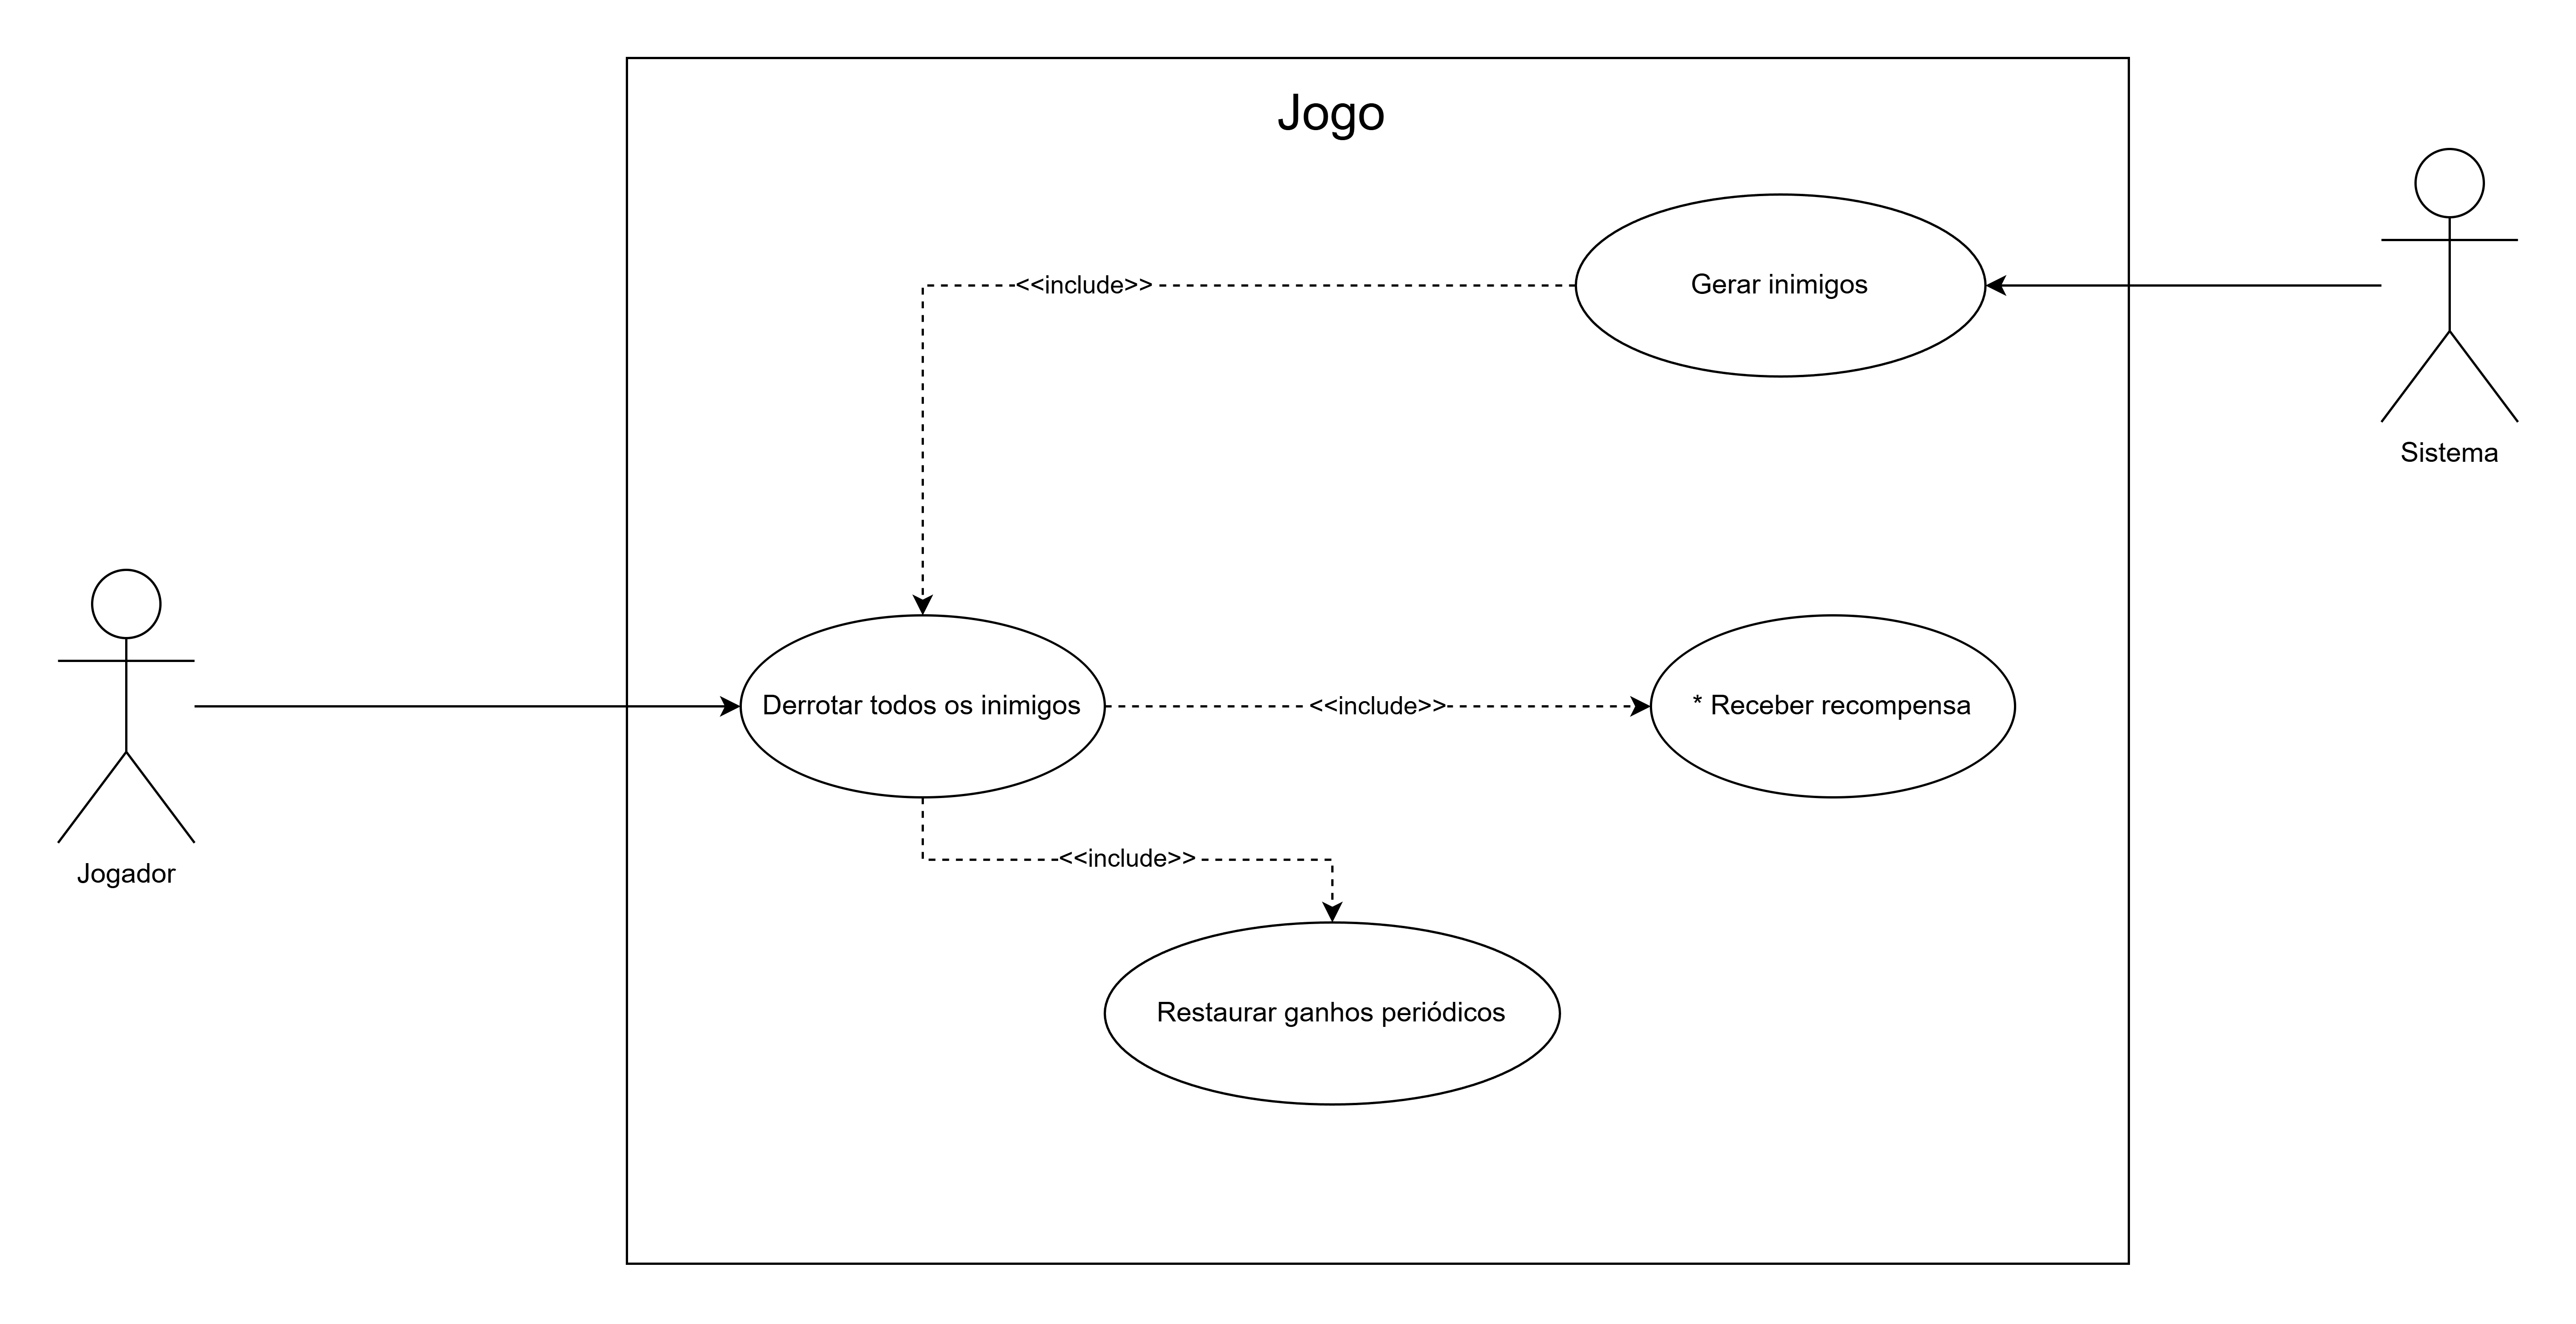
\includegraphics[width=0.9\textwidth]{Diagramas/Use_case_Combate.png}
    \caption{Diagrama de Caso de uso - Combate}
    \label{User_Case_Combat}
\end{figure}

A Figura \ref{User_Case_Combat}, ilustra a interação entre o jogador e o sistema de combate.
Neste sistema, a funcionalidade mais relevante é a "Restaurar ganhos periódicos", uma vez que a partir do momento que o sistema combate "Gera inimigos" os ganhos periódicos são desativados, no entanto,
os custo(prejuízo) não são desativados, o que deixa o jogador numa situação de risco.
O jogador têm de agir rápido para conseguir restaurar os ganhos periódicos, caso contrário, pode perder uma grande quantidade de dinheiro, o que pode levar a uma situação de falência, impossibilitando o pagamento dos custos periódicos, o que leva o jogador a perder o jogo. Esta situação tenta simular o que acontece na relidade, ou seja, quando um data center é atacado pode não conseguir assegurar os seus serviços, resultando em perdas.

\newpage

\section{Implementação}
A implementação constitui a fase em que os planos idealizados são concretizados. 
Nesse sentido, a descrição dos processos será detalhada ao longo desta secção, 
na qual cada subsecção abordará a implementação de uma componente específica 
do projeto.

\subsection{Modelos 3D - Blender}
Dada a natureza do projeto, os modelos 3D assumem um papel de destaque, visto 
que é através destes que o jogador experiencia o mundo e realiza interações. 
Como tal, o seu desenvolvimento deve ser estruturado para maximizar a 
experiência de \textit{gameplay}, mantendo um padrão visual reconhecível e coerente.

Neste sentido, a maioria dos modelos 3D foi desenvolvida por autoria própria, 
recorrendo ao \textit{software} Blender.

\newpage

\subsubsection{Cenário}

\begin{figure}[H]
     \centering
     % Primeira Foto
     \begin{subfigure}[b]{0.3\textwidth}
         \centering
         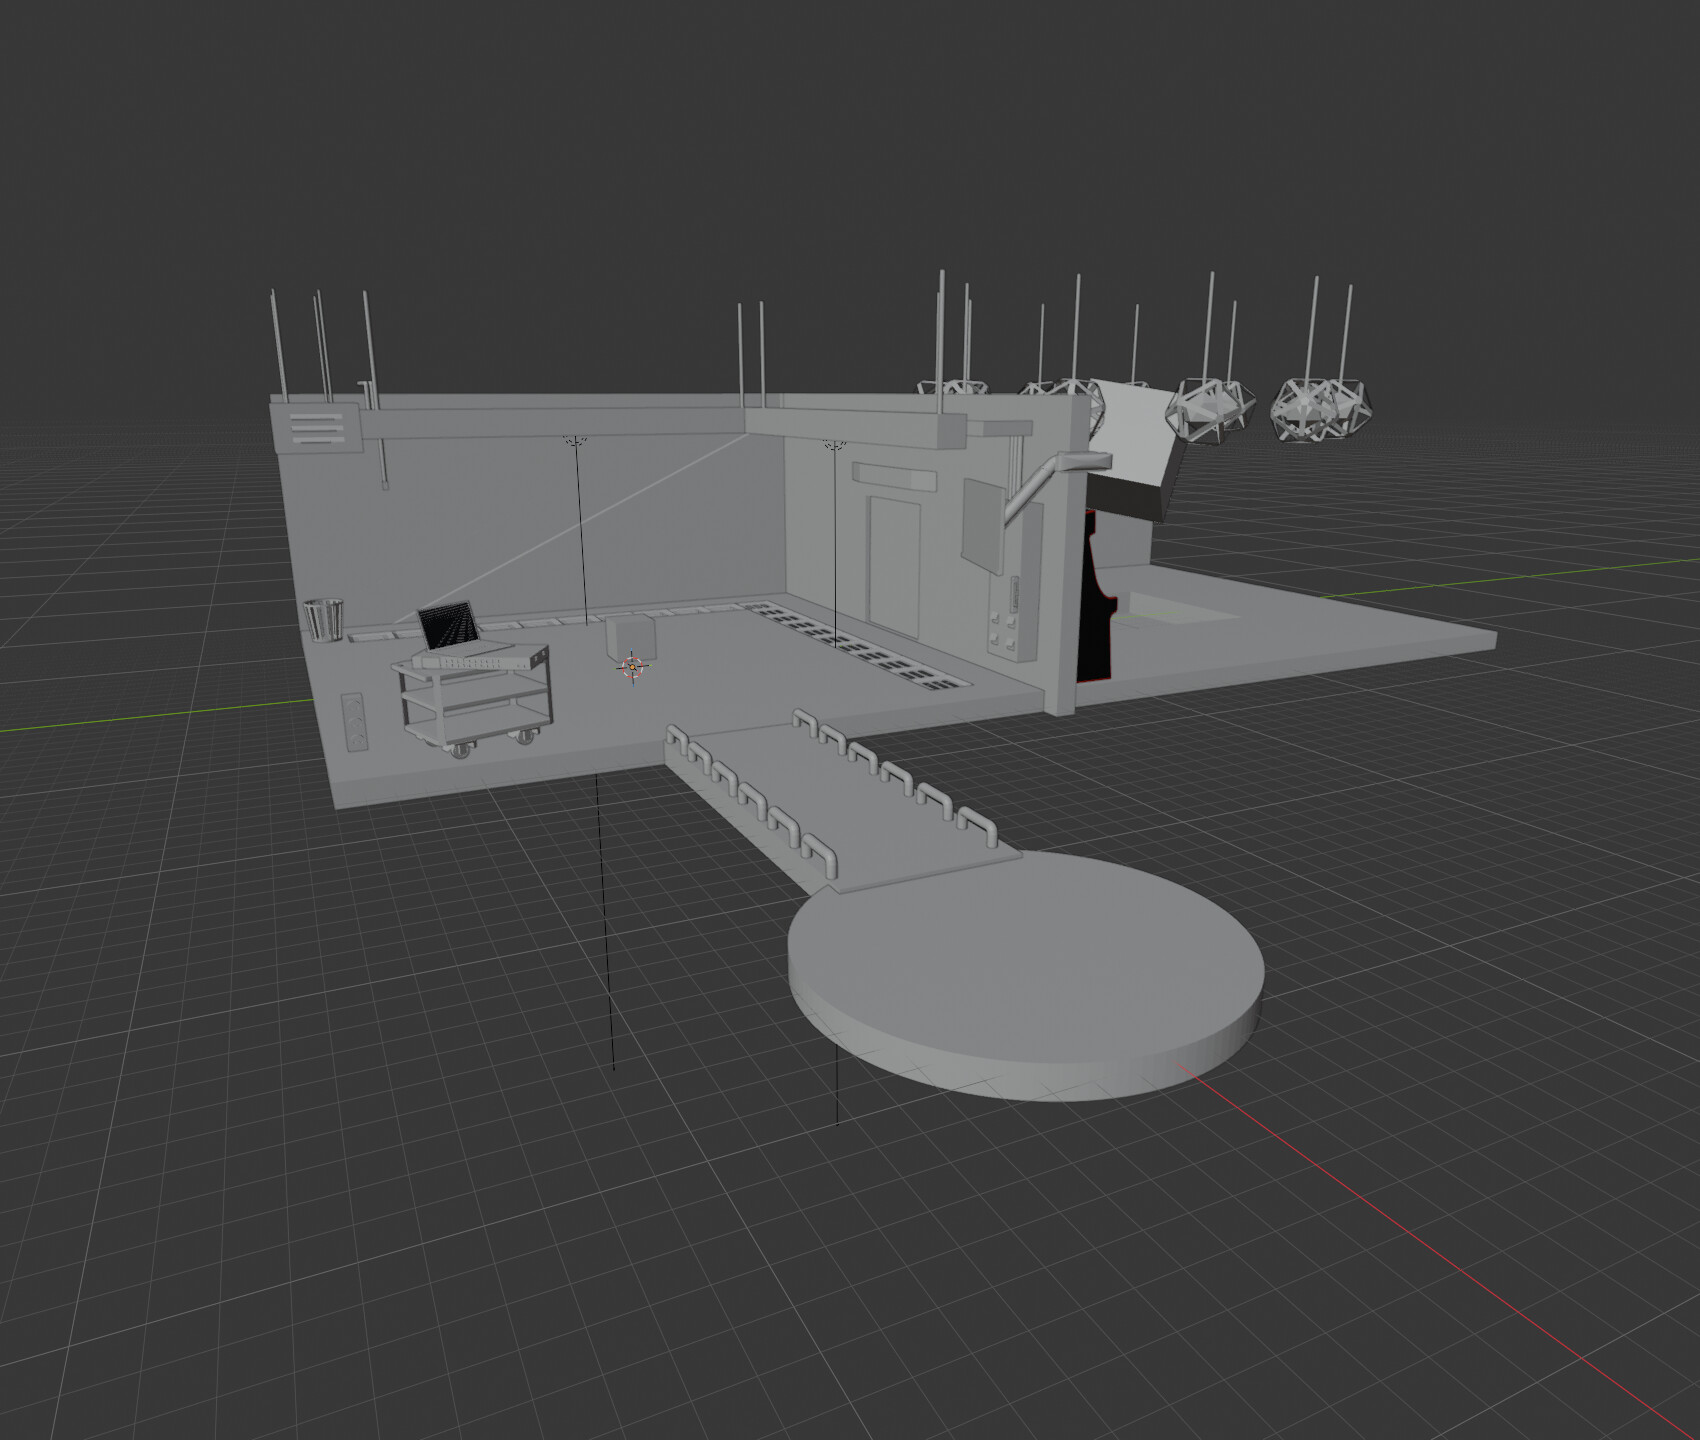
\includegraphics[width=\textwidth]{Blender/CenarioViewPort1.jpg}
         \caption{Cenário Vista de \textit{ViewPort} 1}
         \label{fig:foto1}
     \end{subfigure}
     \hfill
     % Segunda Foto
     \begin{subfigure}[b]{0.3\textwidth}
         \centering
         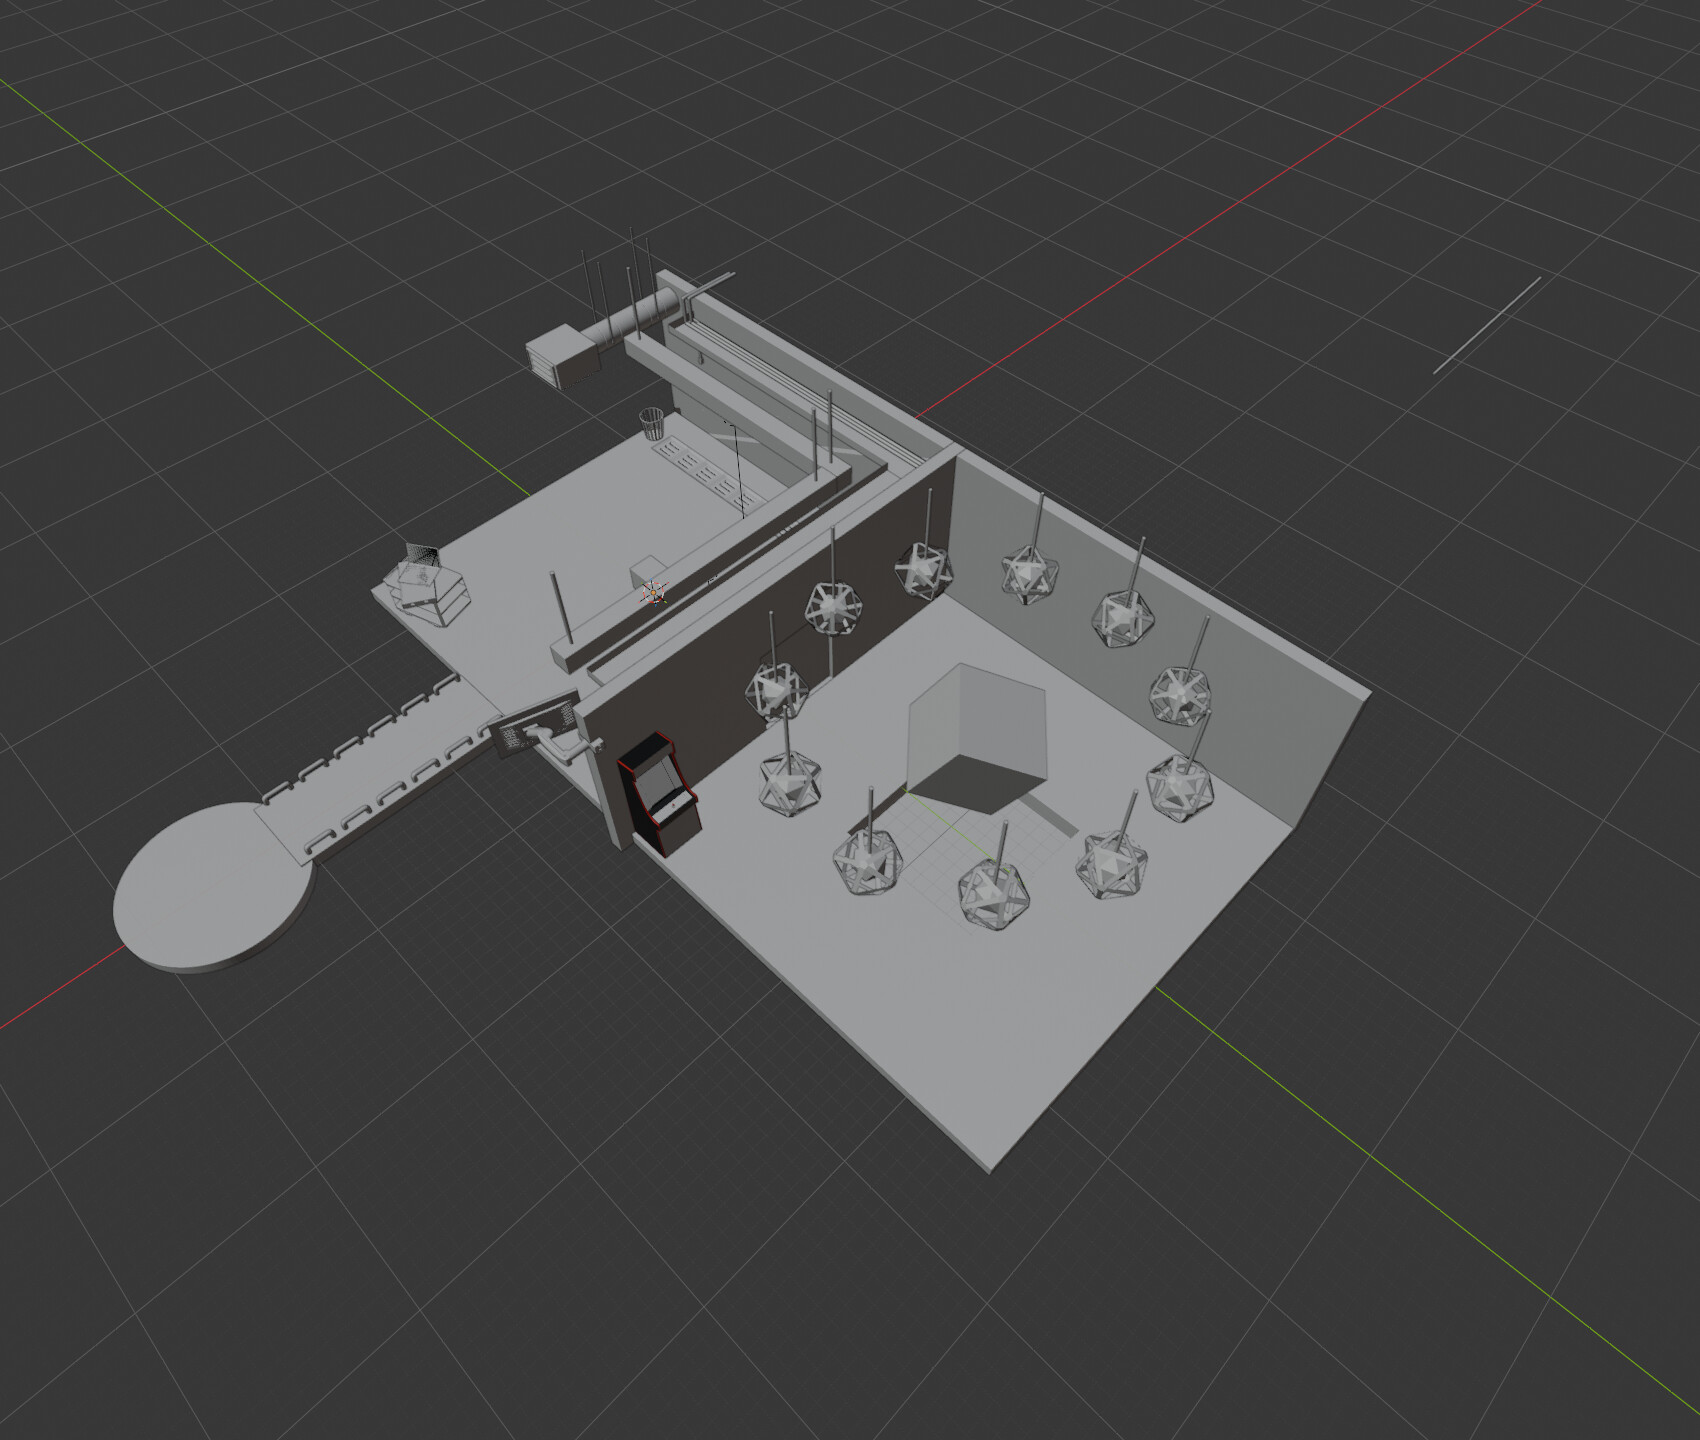
\includegraphics[width=\textwidth]{Blender/CenarioViewPort2.jpg}
         \caption{Cenário Vista de \textit{ViewPort} 2}
         \label{fig:foto2}
     \end{subfigure}
     \hfill
     % Terceira Foto
     \begin{subfigure}[b]{0.3\textwidth}
         \centering
         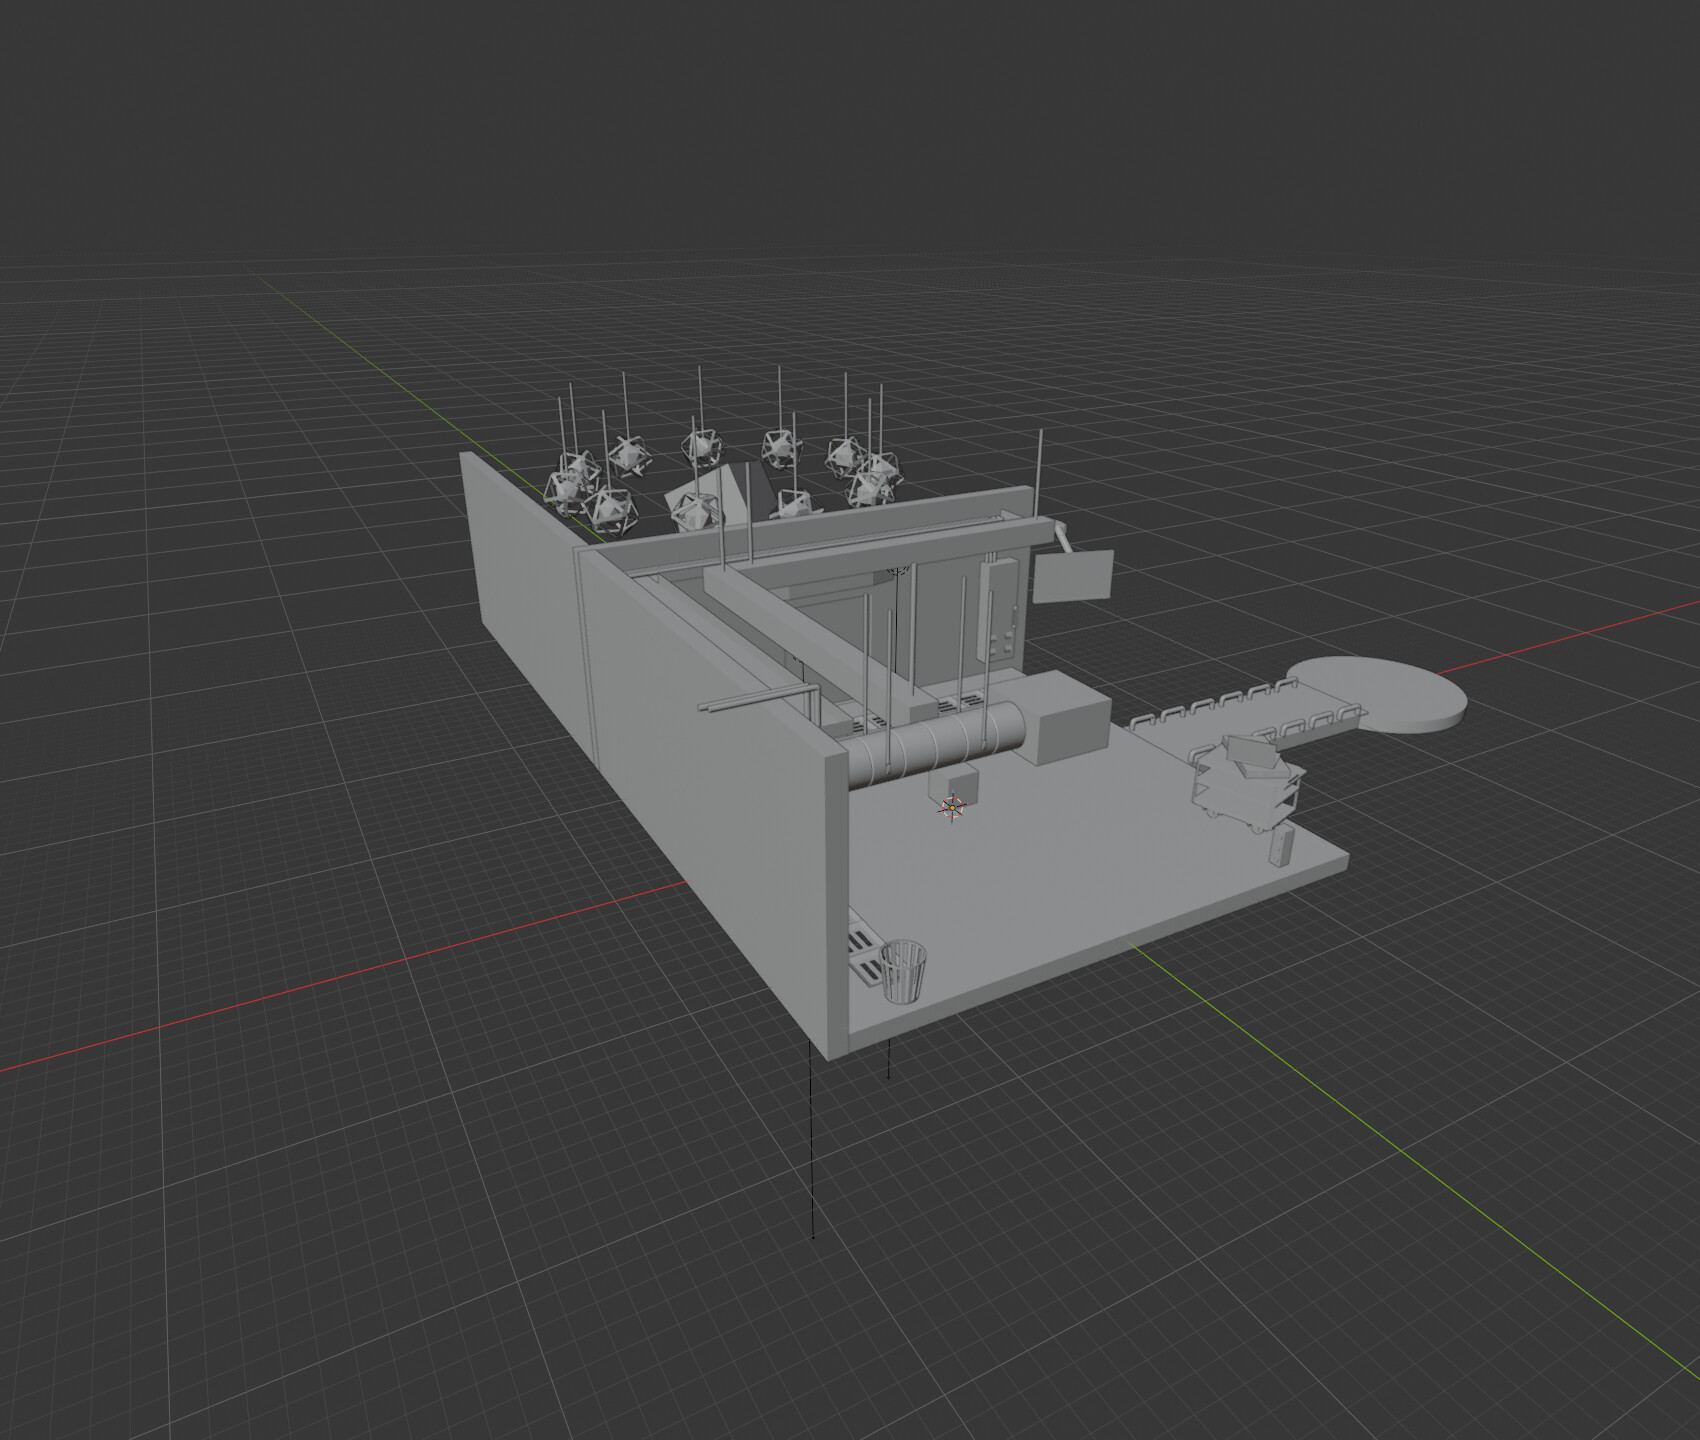
\includegraphics[width=\textwidth]{Blender/CenarioViewPort3.jpg}
         \caption{Cenário Vista de \textit{ViewPort} 3}
         \label{fig:foto3}
     \end{subfigure}
     
     \caption{Vistas de \textit{ViewPort} do cenário.}
     \label{CenarioViewportGroup3.1}
\end{figure}

\begin{figure}[H]
    \centering
    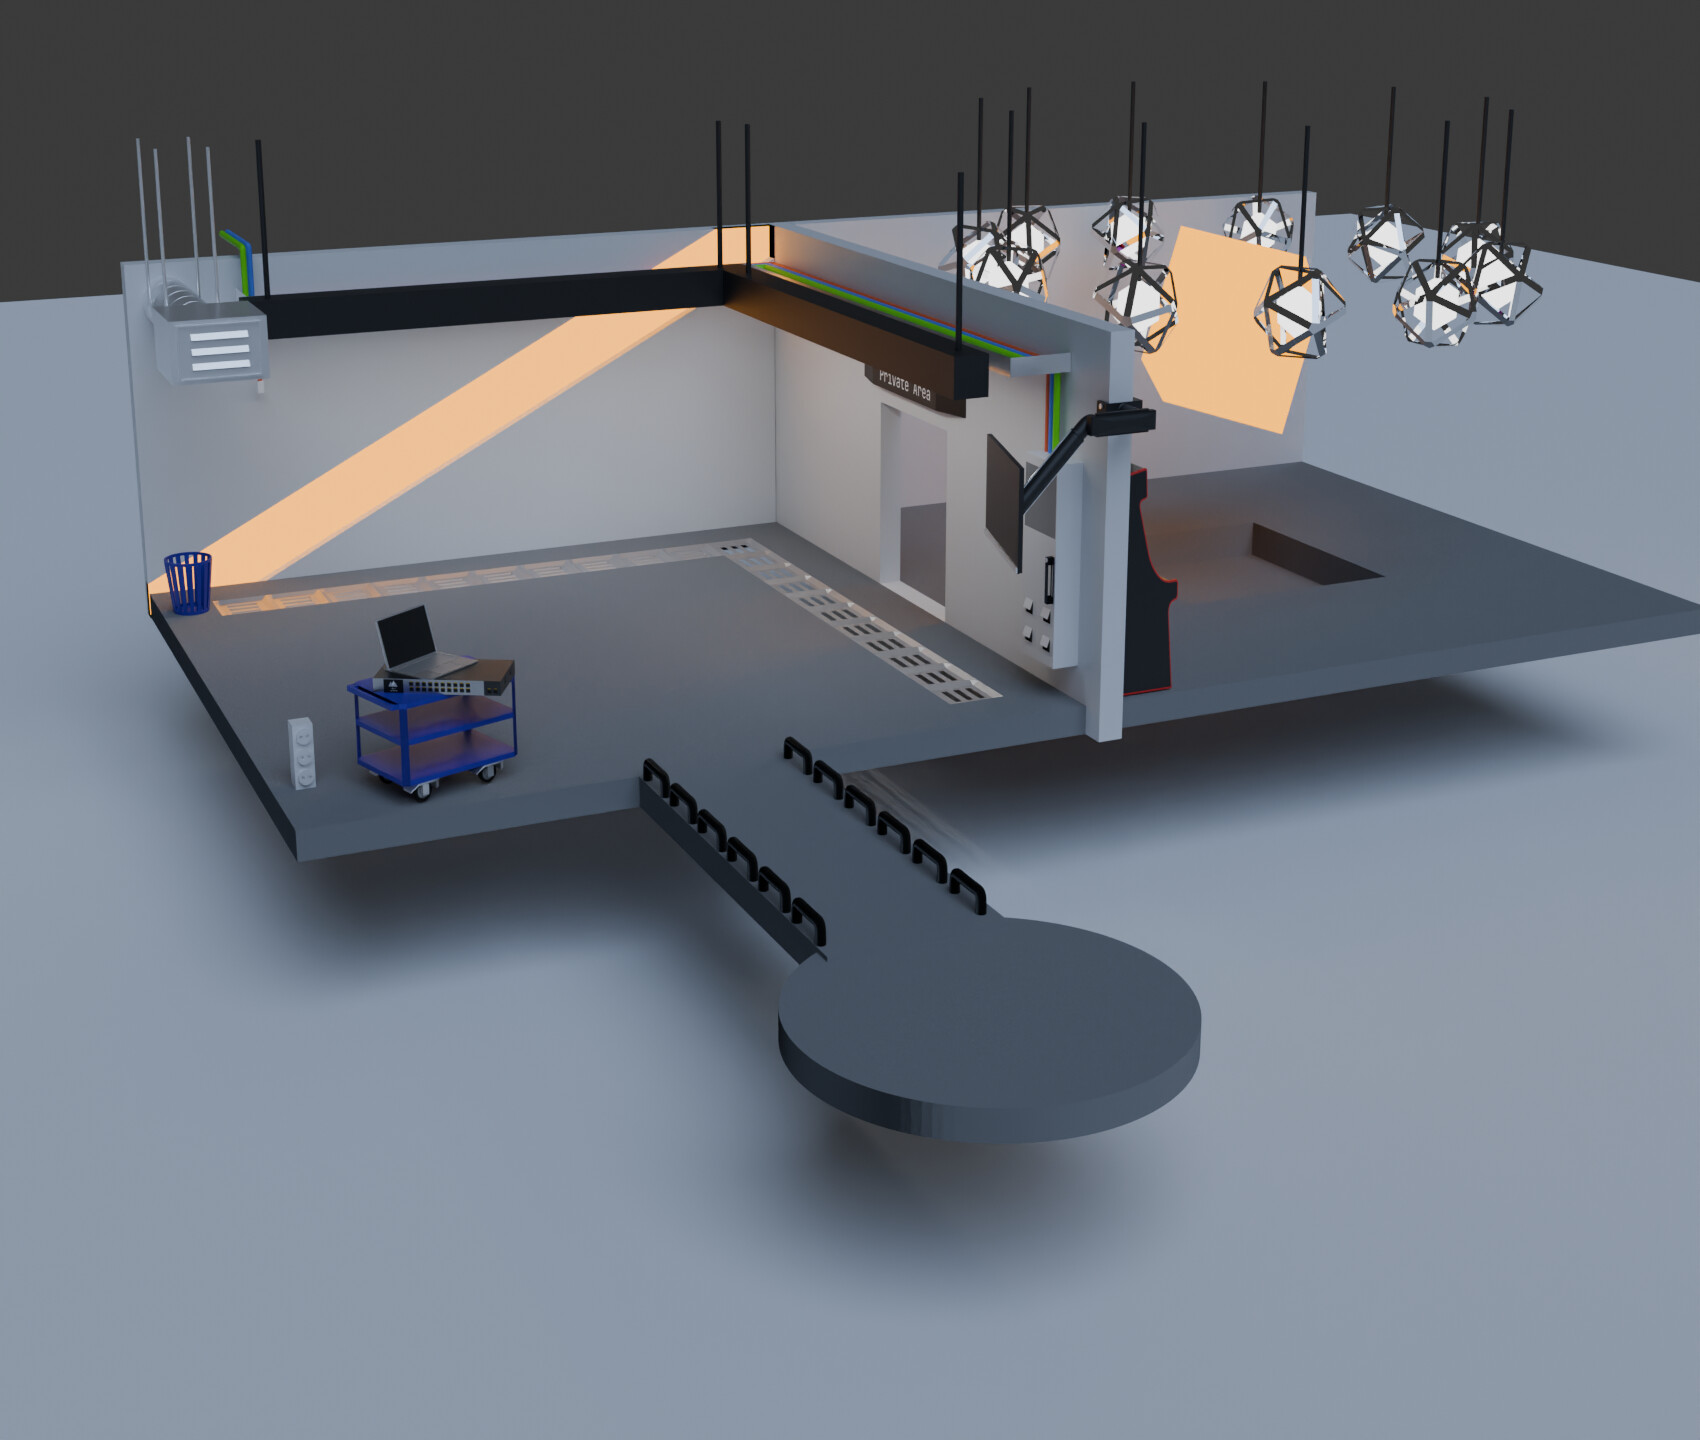
\includegraphics[width=0.65\textwidth]{Blender/CenárioRender.jpg}
    \caption{Vista renderizada do cenário do jogo.}
    \label{CenarioRender1}
\end{figure}

As Figuras \ref{CenarioViewportGroup3.1} e \ref{CenarioRender1}
ilustra o trabalho desenvolvido para o cenário.
Todos os subcomponentes dos cenários, tais como, mesas, computadores, e outros detalhes
desenvolvidos com a ajuda do \textit{software}.

\newpage

\subsubsection{Canhão}
\label{Sec:Canhão}

\begin{figure}[H]
     \centering
     % Primeira Foto
     \begin{subfigure}[b]{0.3\textwidth}
         \centering
         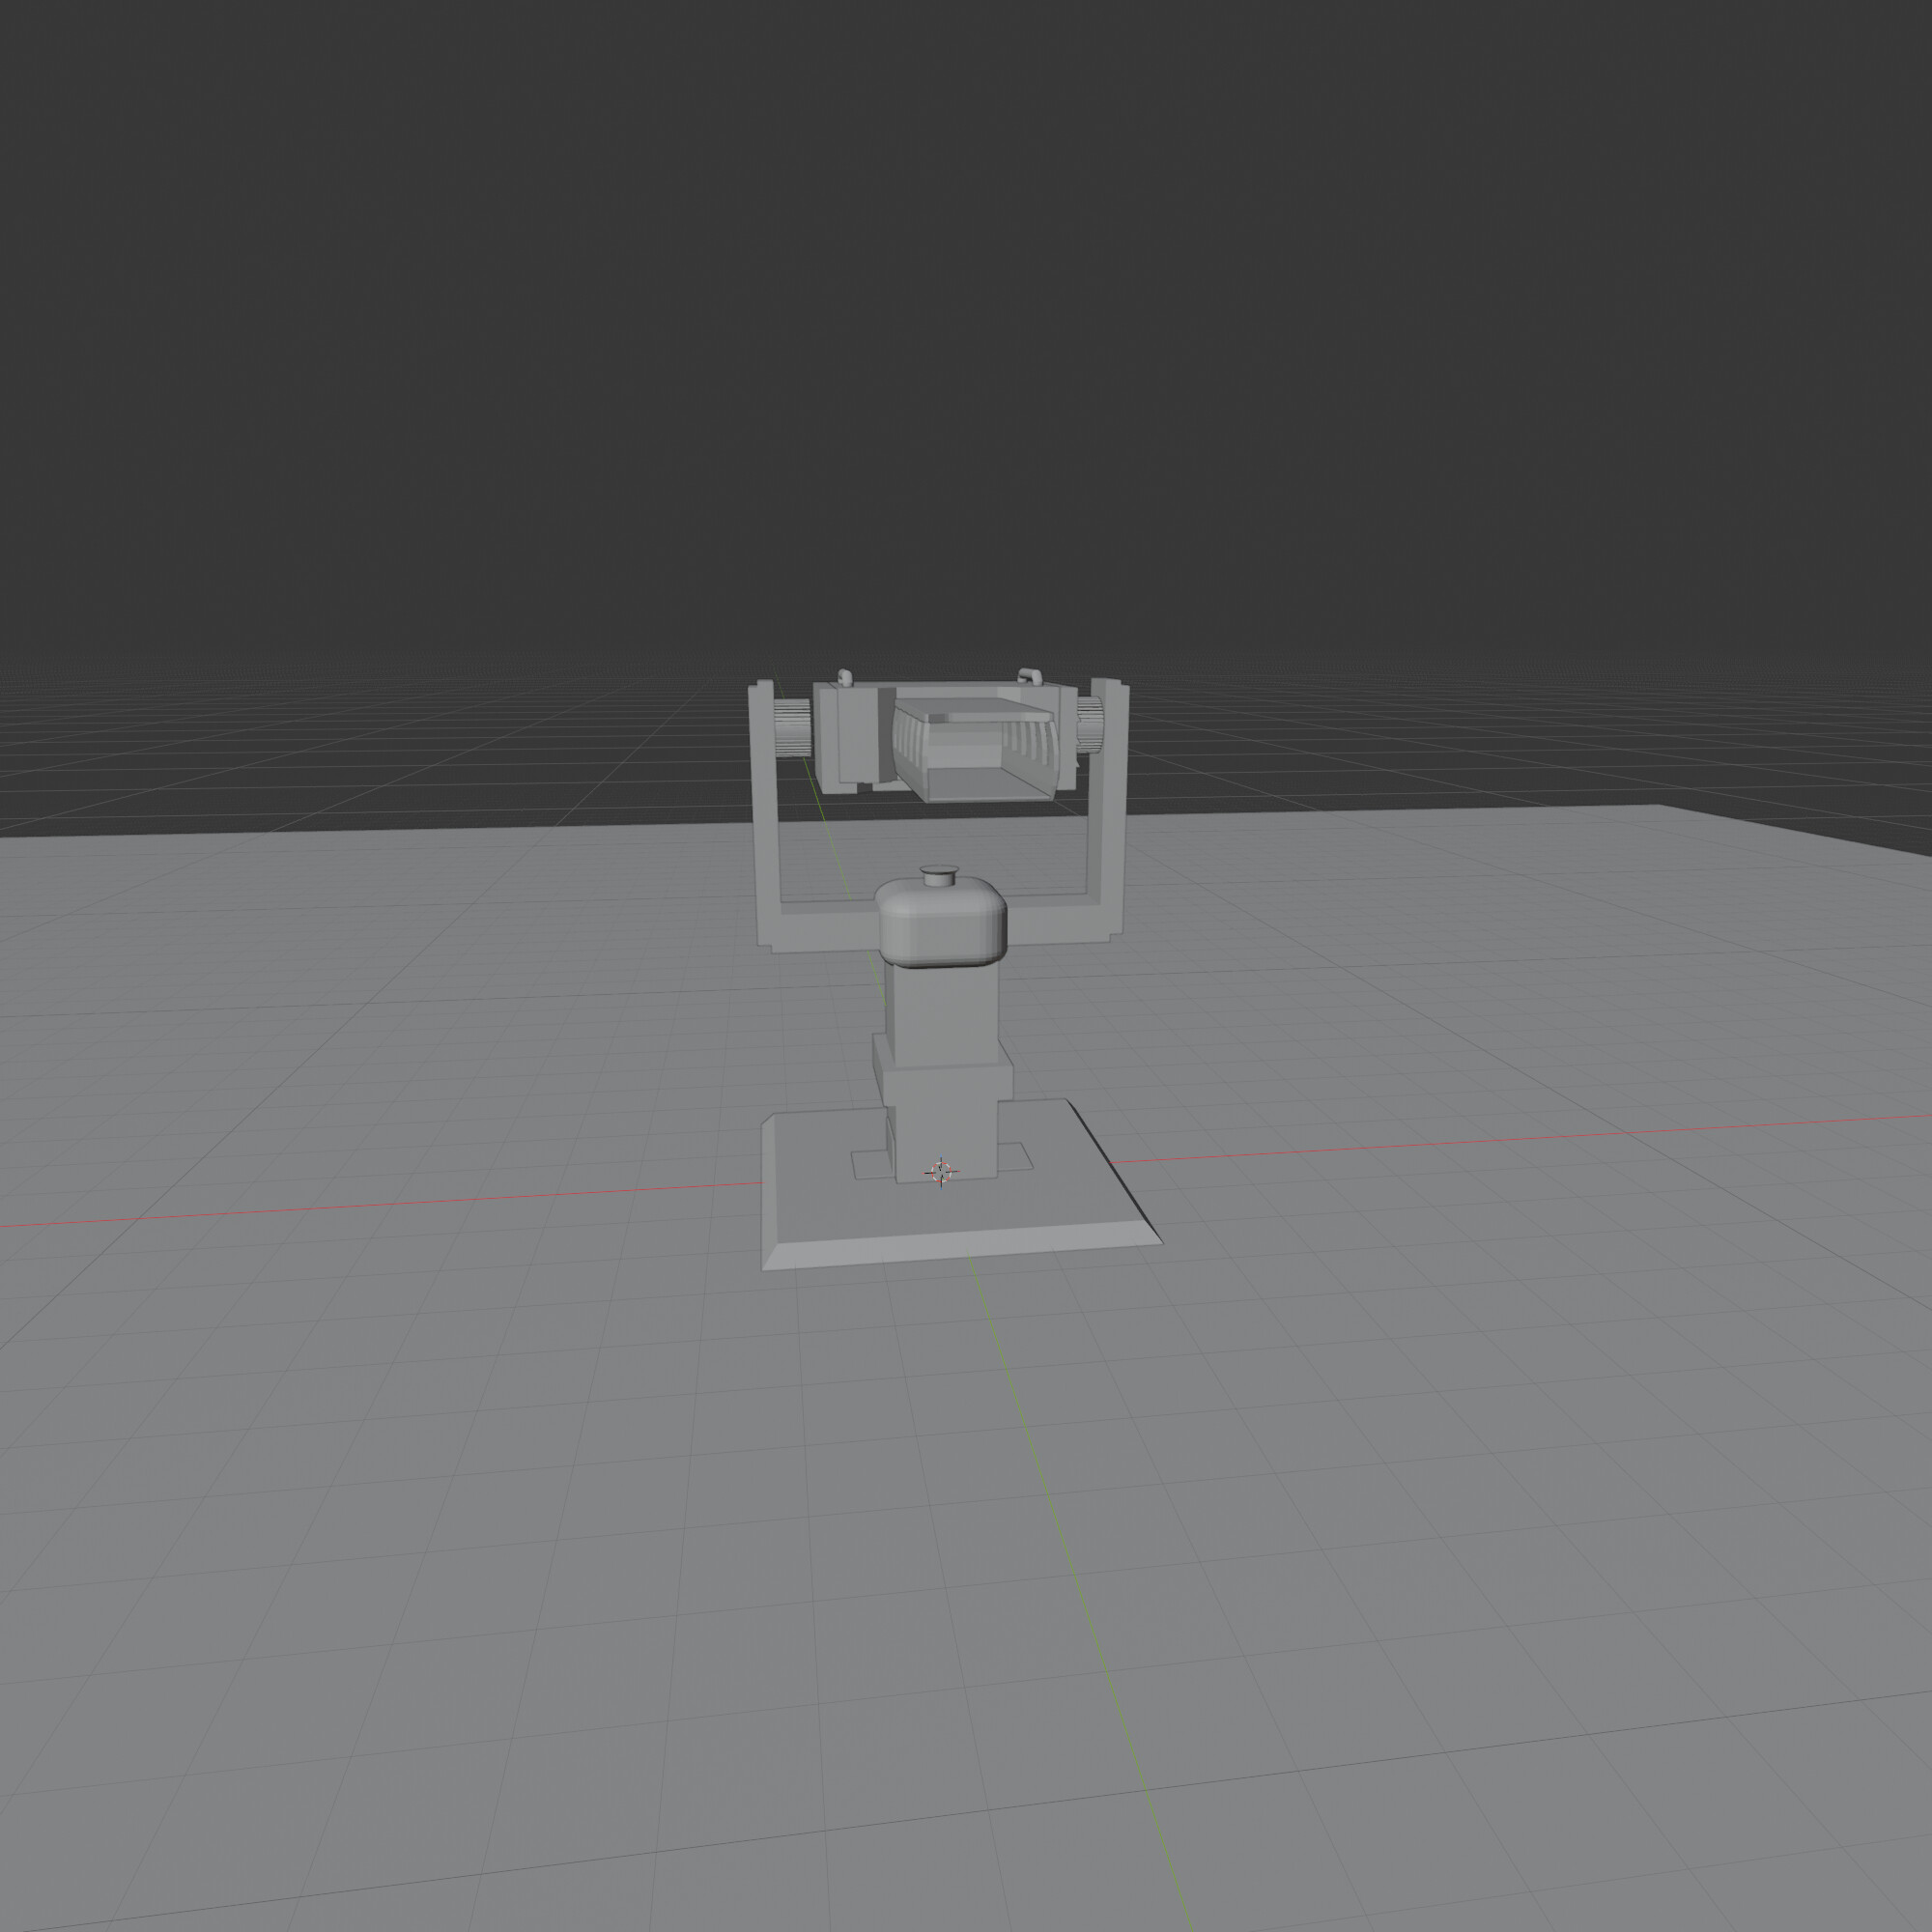
\includegraphics[width=\textwidth]{Blender/CanhaoViewPort1.jpg}
         \caption{Cenário Vista de \textit{ViewPort} 1}
         \label{fig:foto1Canhao}
     \end{subfigure}
     \hfill
     % Segunda Foto
     \begin{subfigure}[b]{0.3\textwidth}
         \centering
         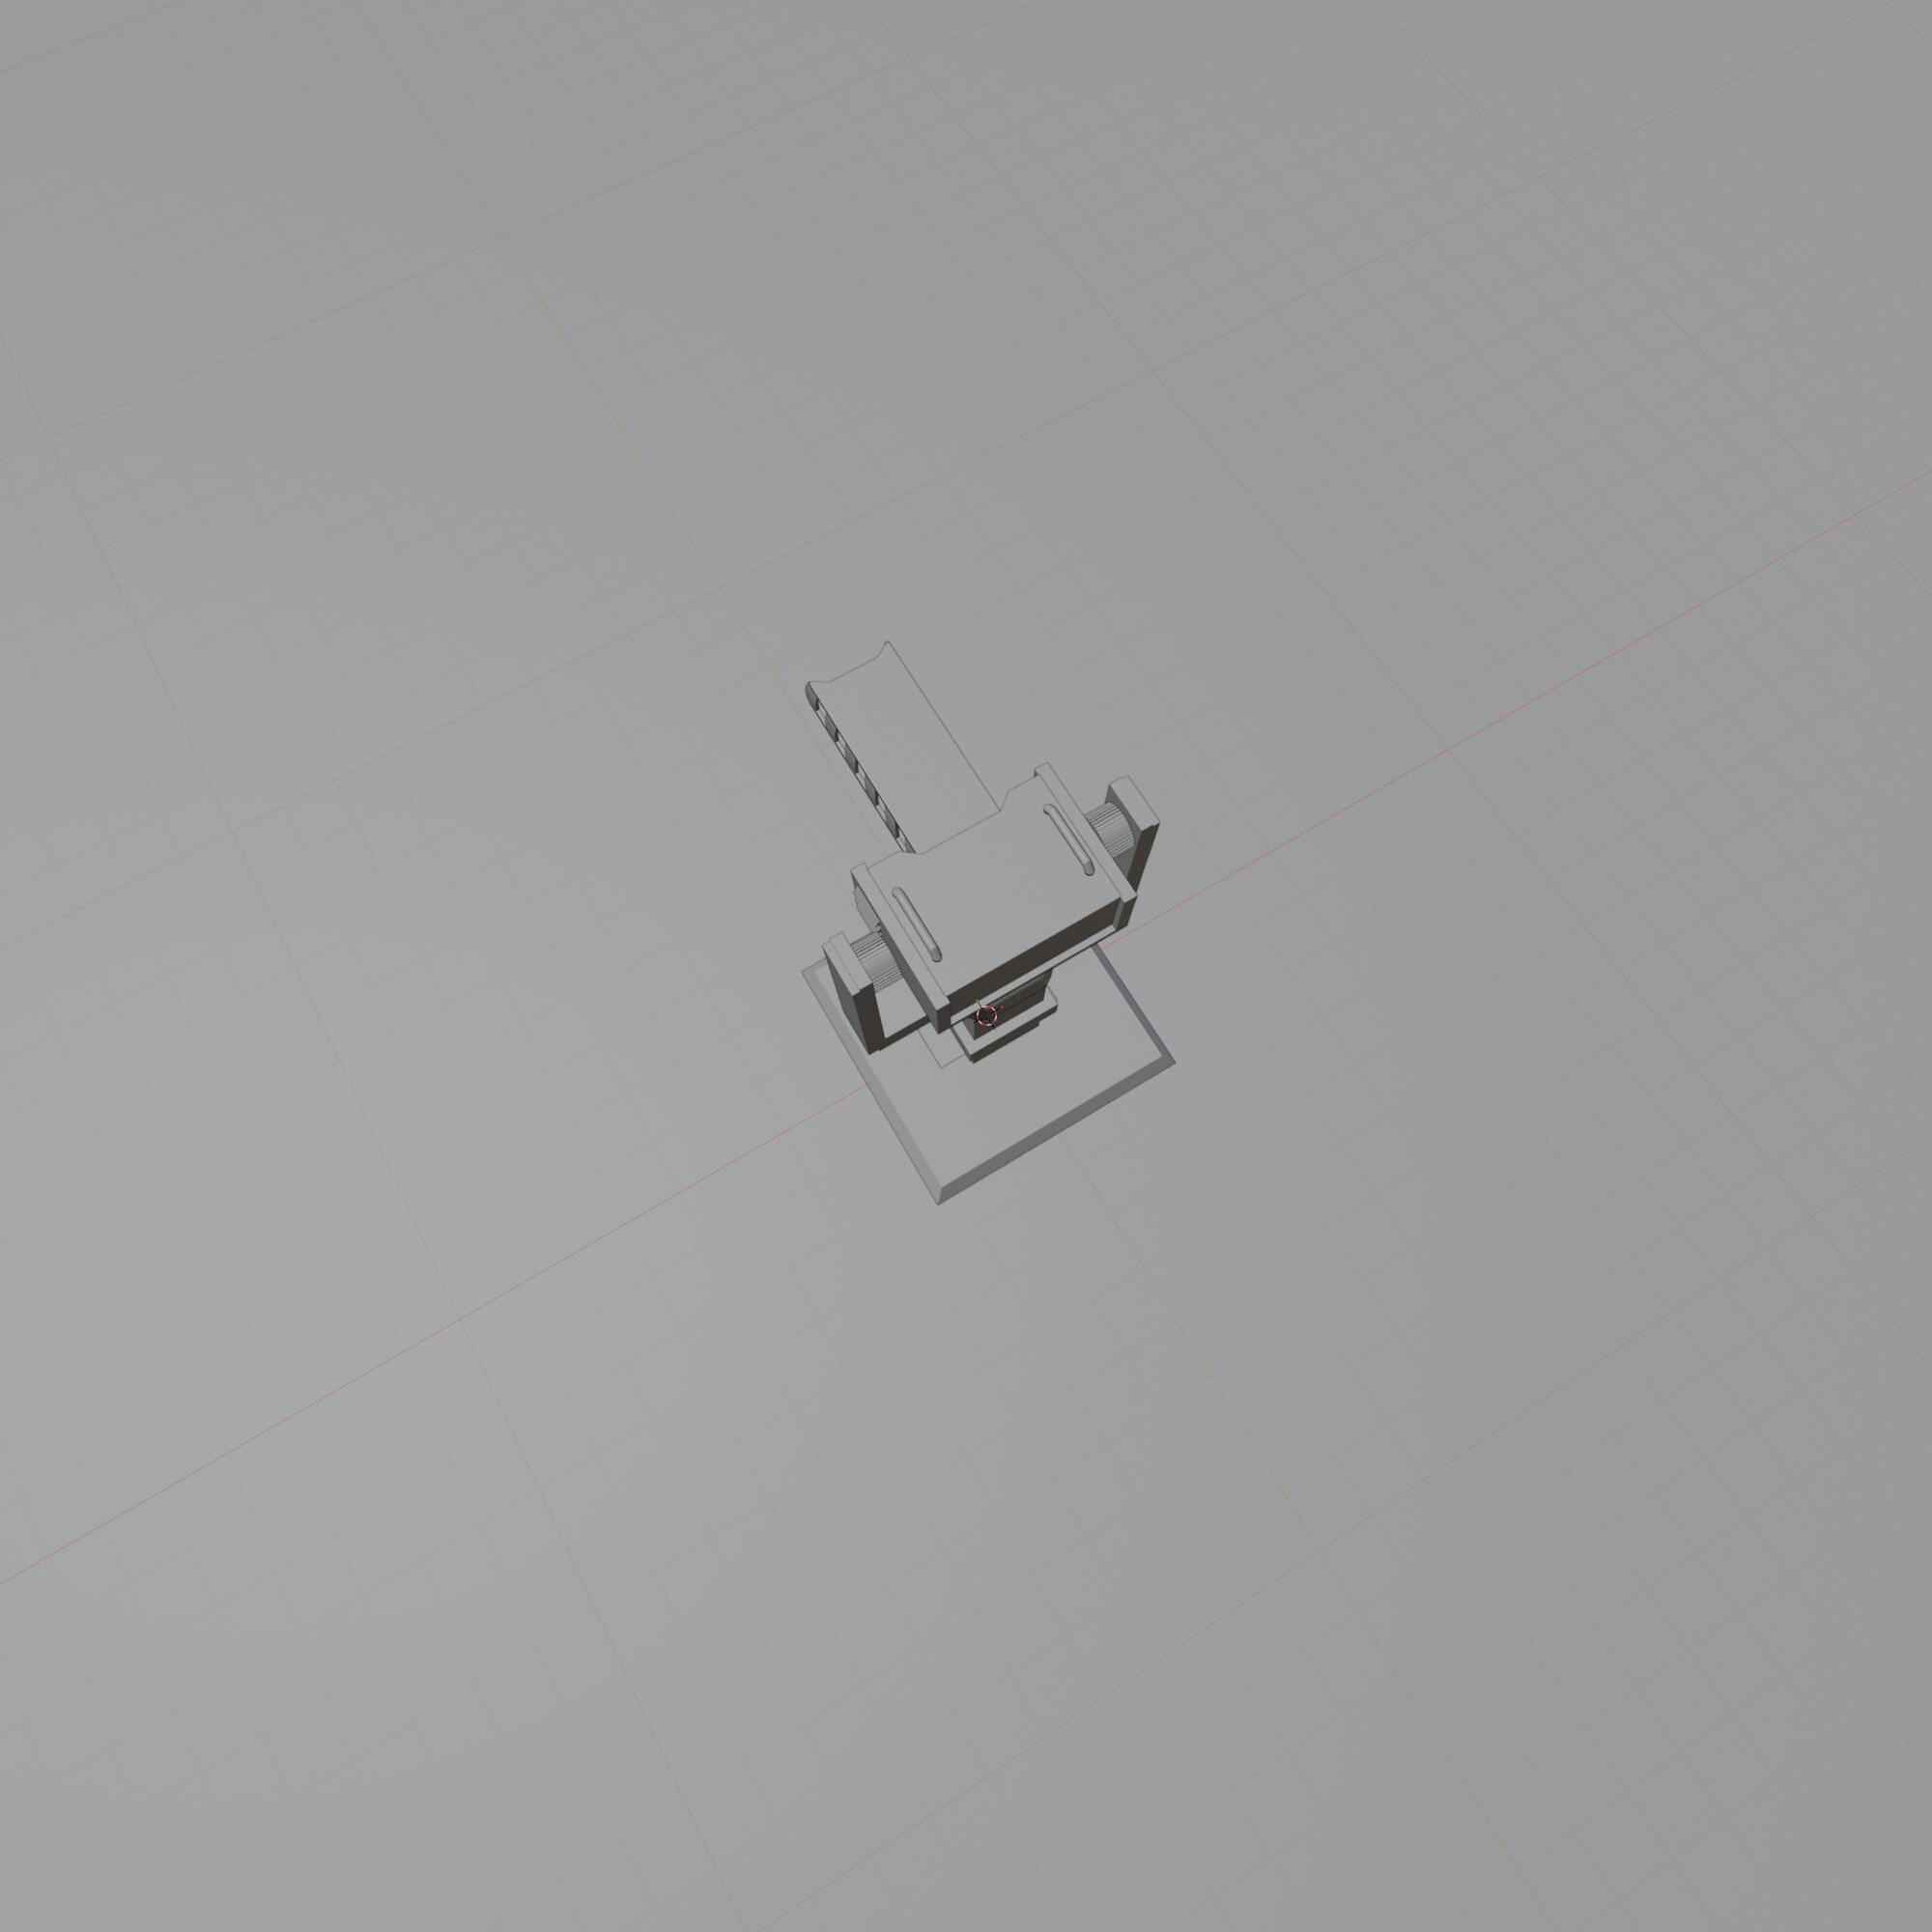
\includegraphics[width=\textwidth]{Blender/CanhaoViewPort2.jpg}
         \caption{Cenário Vista de \textit{ViewPort} 2}
         \label{fig:foto2Canhao}
     \end{subfigure}
     \hfill
     % Terceira Foto
     \begin{subfigure}[b]{0.3\textwidth}
         \centering
         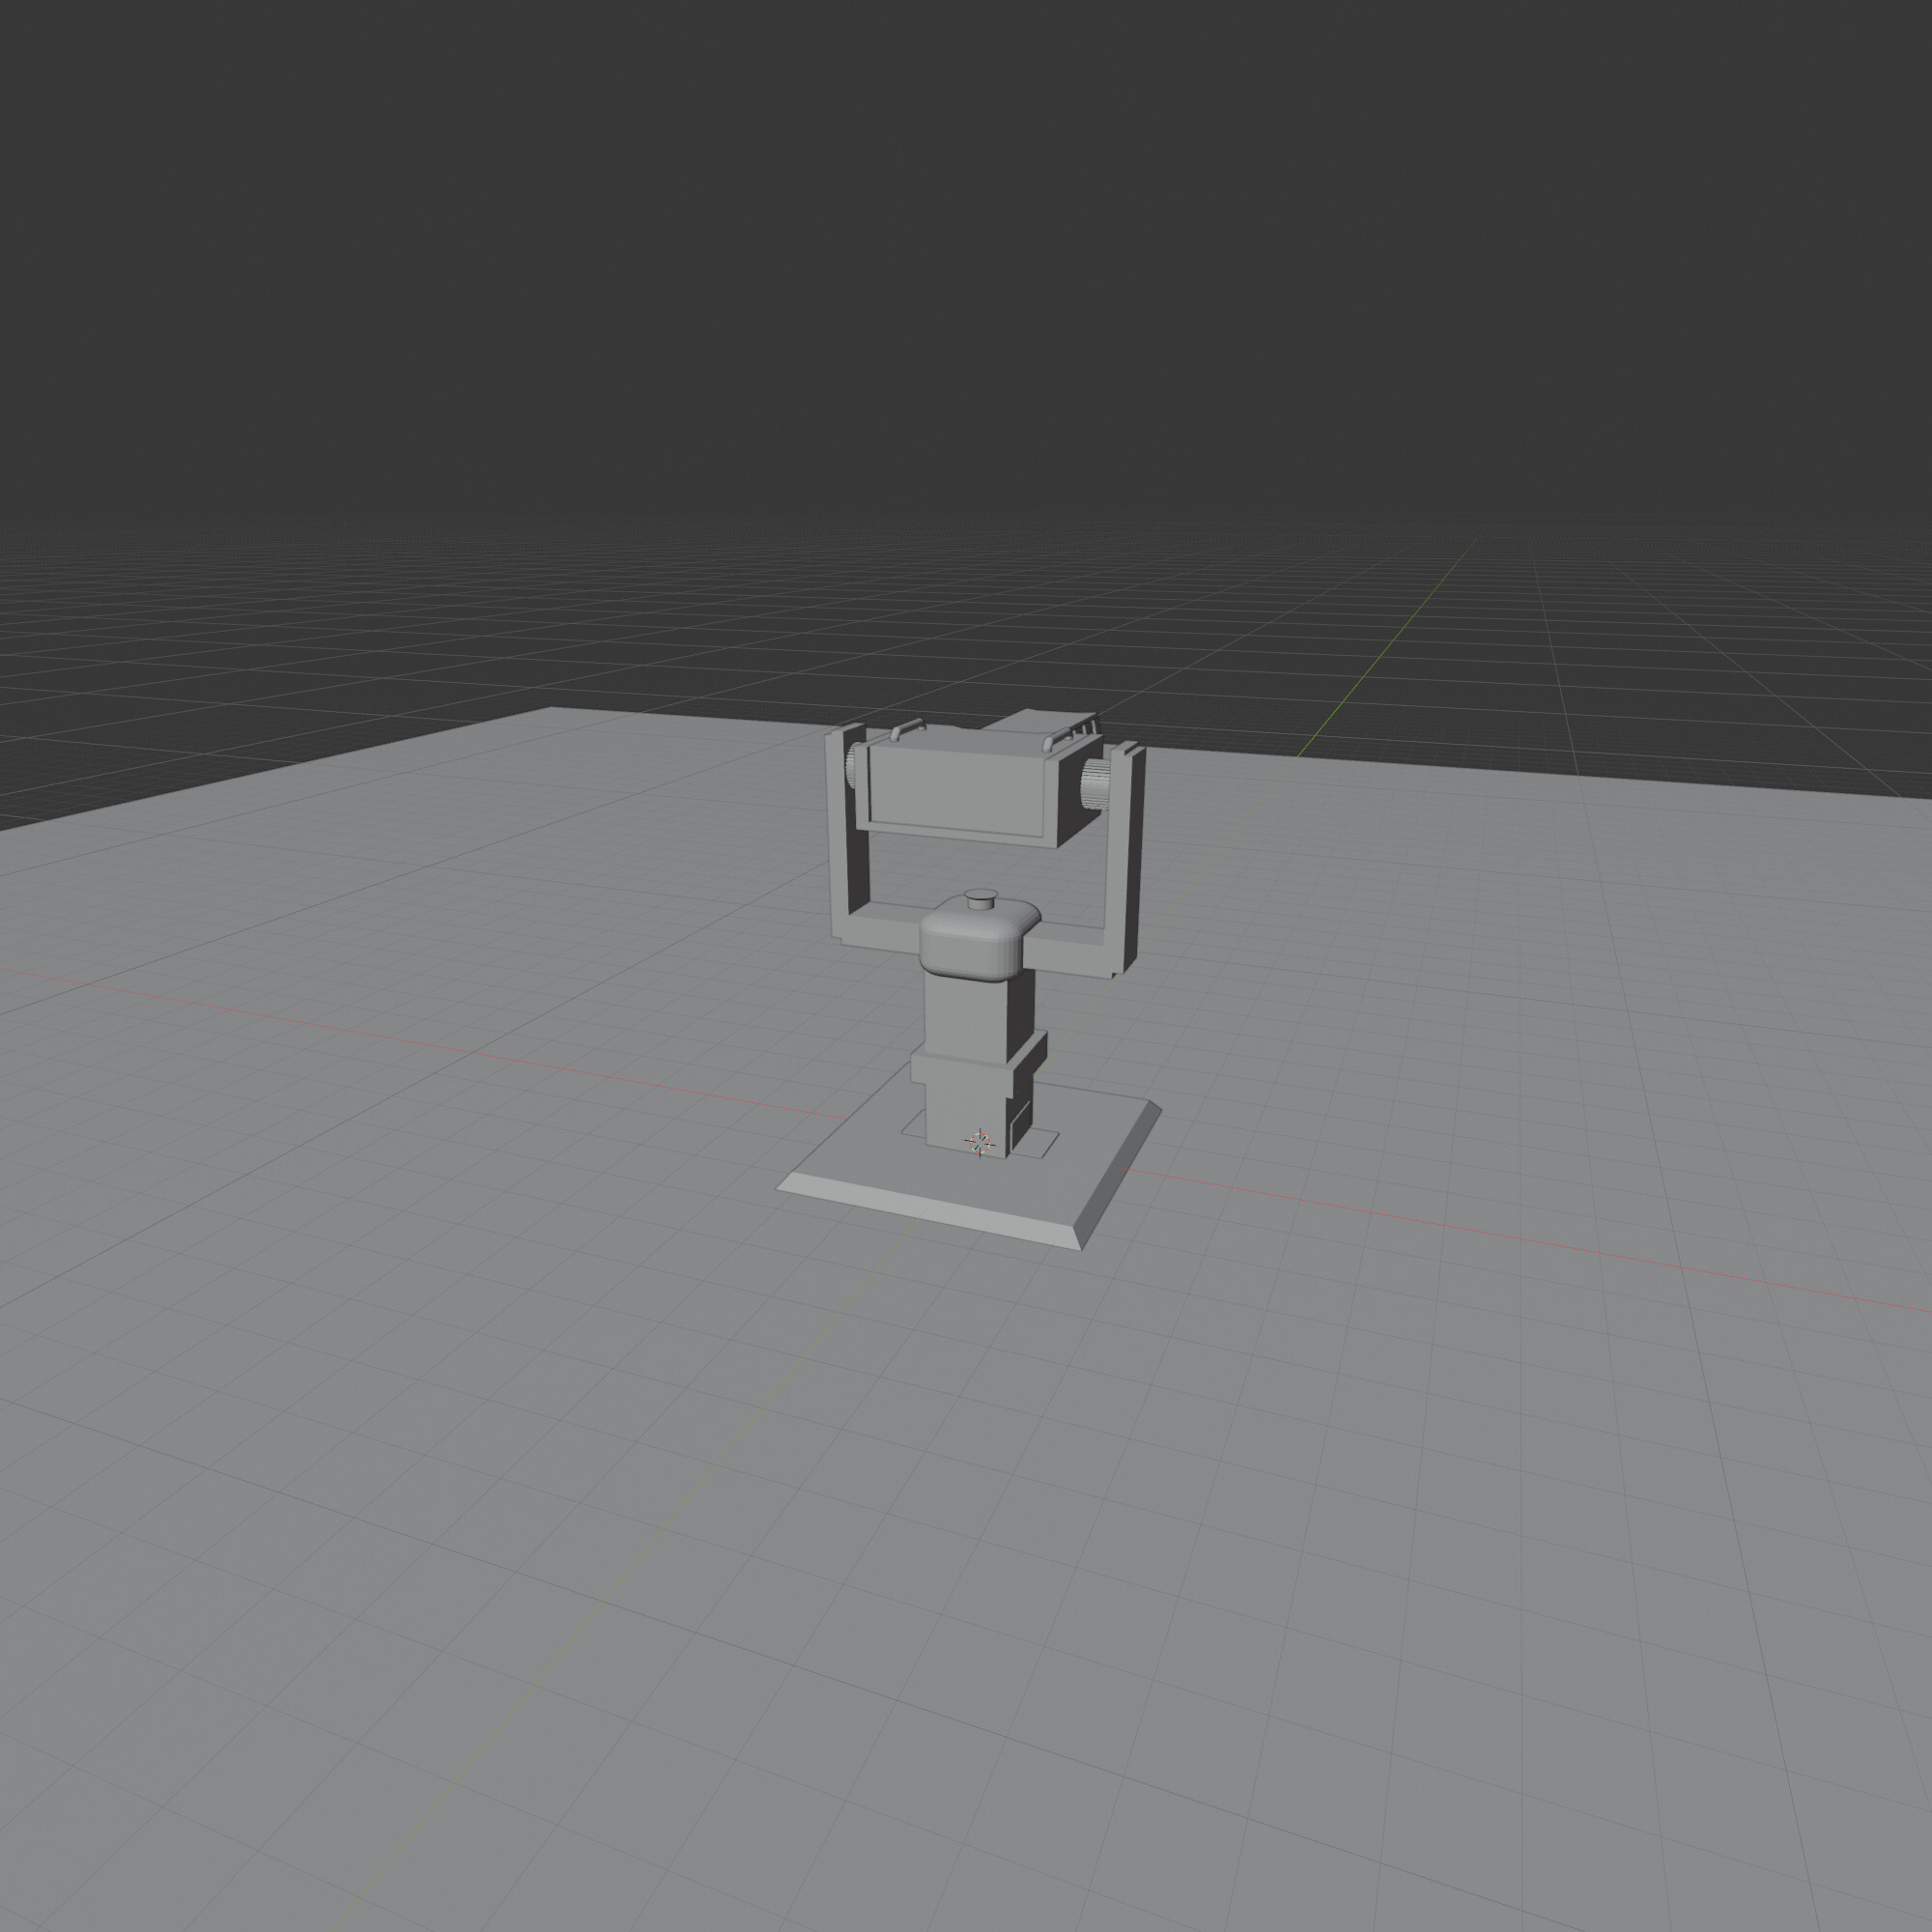
\includegraphics[width=\textwidth]{Blender/CanhaoViewPort3.jpg}
         \caption{Cenário Vista de \textit{ViewPort} 3}
         \label{fig:foto3Canhao}
     \end{subfigure}
     
     \caption{Vistas de \textit{ViewPort} do canhão.}
     \label{CanhaoViewportGroup3.1}
\end{figure}

\begin{figure}[H]
    \centering
    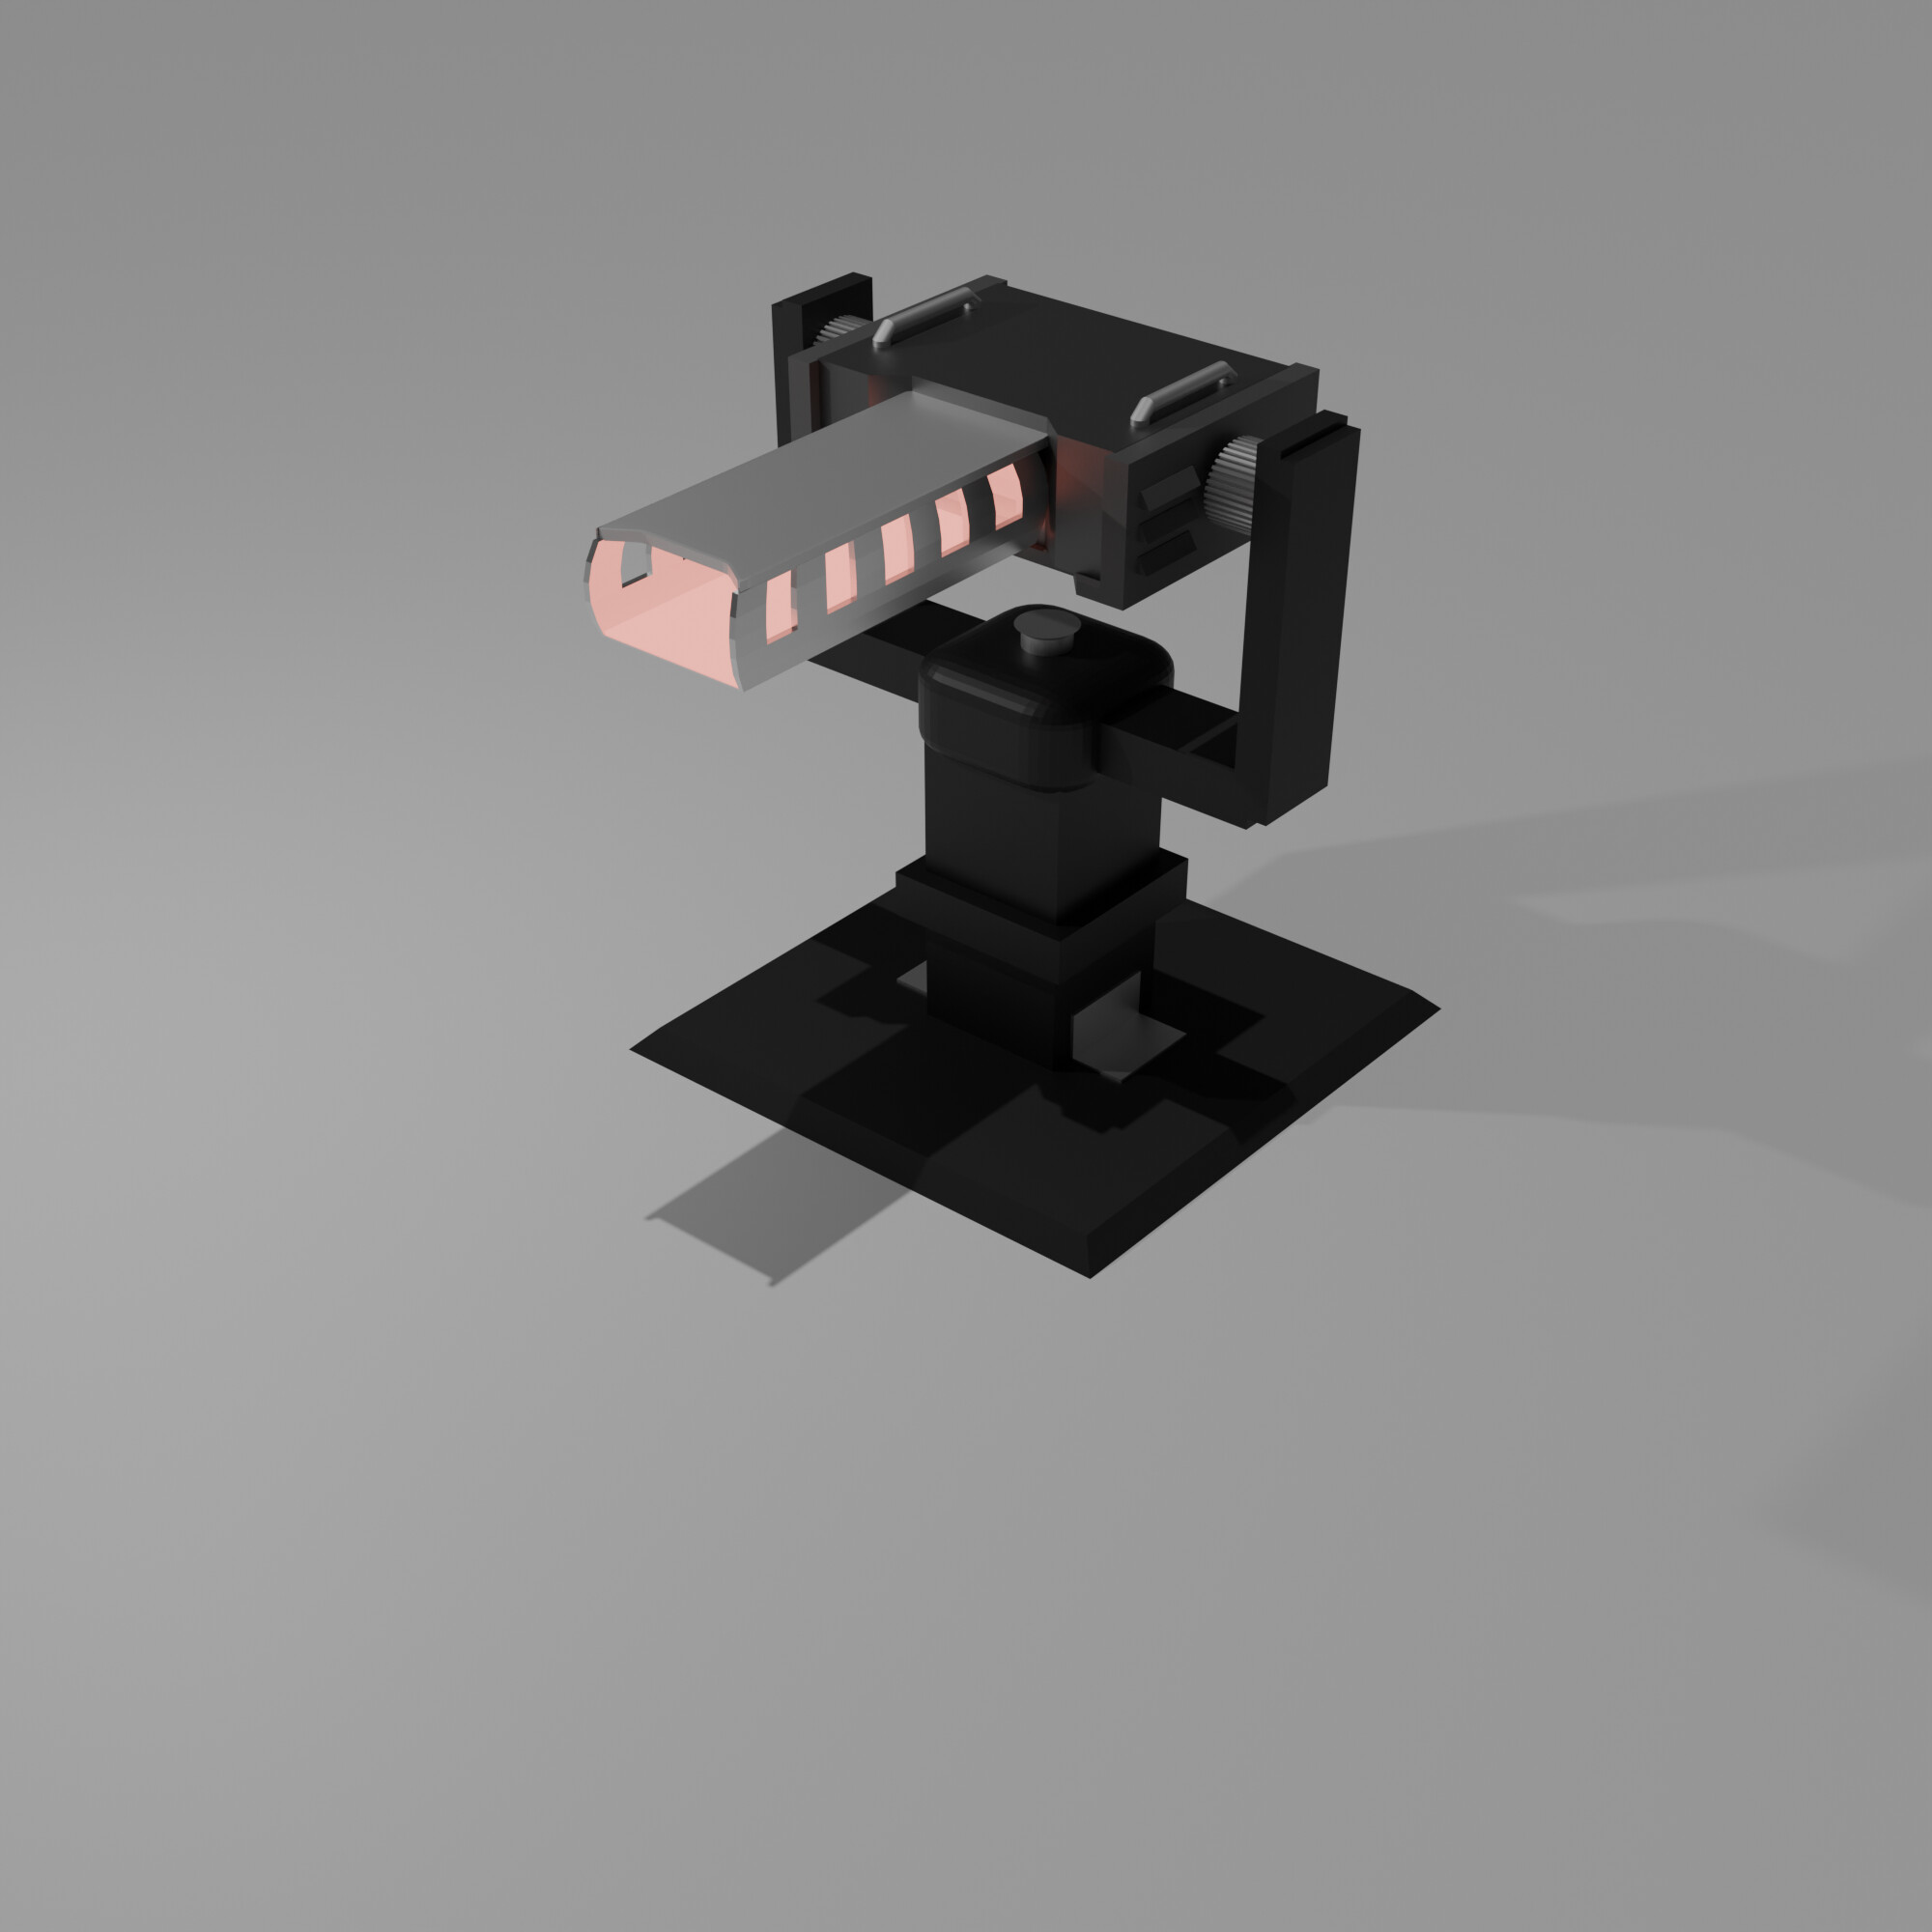
\includegraphics[width=0.55\textwidth]{Blender/CanhaoRender.jpg}
    \caption{Vista renderizada do canhão.}
    \label{CanhaoRender1}
\end{figure}

As Figuras \ref{CanhaoViewportGroup3.1} e \ref{CanhaoRender1} ilustram
o modelo do canhão. Os processos de modelação assim como de pintura 
de materiais, foram desenvolvidos dentro do \textit{software} Blender.

Com o design deste modelo, pretenda-se transmitir uma sensação de 
futurismo moderada, 
mas que, ao mesmo tempo, harmozine com o cenário restante.

\subsection{Imagens e \textit{assets} 2D}

Embora não sejam tão utilizados quanto os ativos 3D, os ativos 
2D apresentam um papel bastante importante, sobretudo para elementos
de \ac{UI} e para a idealização do contexto de elementos.

\subsubsection{Idealização do personagem}

\begin{figure}[H]
    \centering
    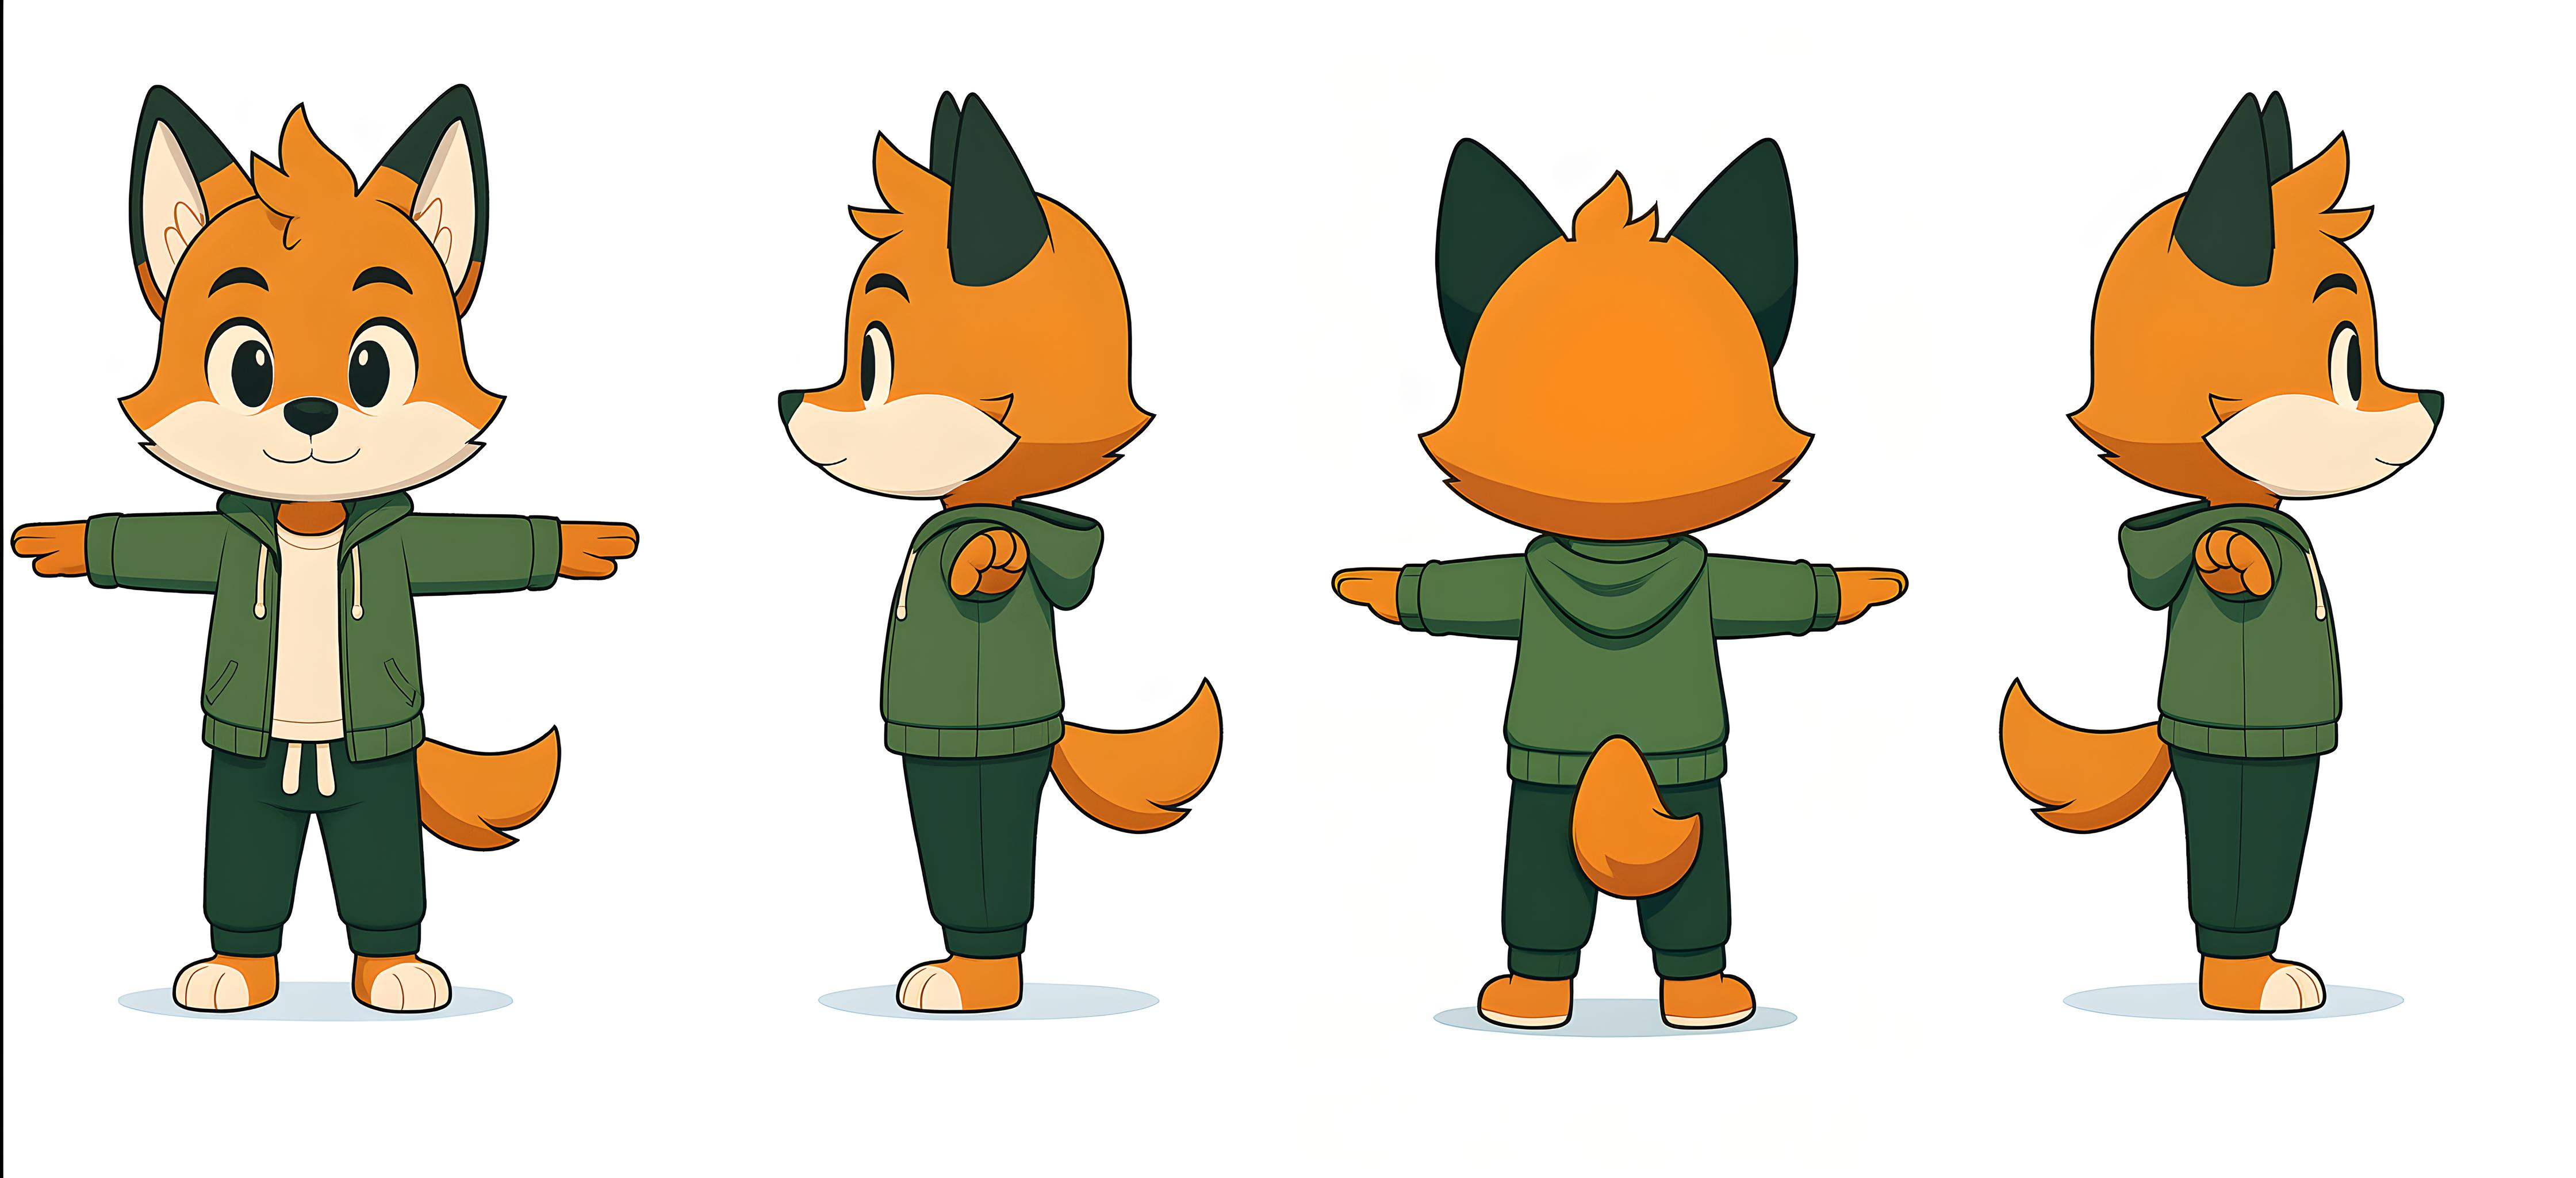
\includegraphics[width=0.8\textwidth]{images/Character_image.jpg}
    \caption{Ilustração do personagem feita com o uso da \ac{IA} - Nano Banana (Gemini)}
    \label{idealizacaoCharacter}
\end{figure}

Durante o processo criativo do personagem, utilizou-se a ferramenta 
Nano Banana do Gemini para gerar a Figura \ref{idealizacaoCharacter}. 
O objetivo foi representar visualmente as suas características físicas, 
de maneira que, esta possa ser utilizada por outras ferramentas de IA, 
tais como o Chat 3D, para a criação de um modelo tridimensional.

\subsubsection{\textit{Frames} para a criação de animações 2D}

No contexto de jogos de vídeo, transmitir \textit{feedbacks} ao jogador
é um dos processos mais importantes, uma vez que eles funcionam como uma
confirmação que uma ação foi realizada e/ou ajudam a construir a experiência
facilitando a evocação de emoções para jogador.

\textit{Feedbacks} podem ser transmitidos, através de \ac{VFX}, animações e efeitos sonoros,
por exemplo, efeitos visuais de faíscas no disparo de uma arma, até animações
do personagem a andar, etc\dots

Posto isto, para a construção de certos \textit{feedbacks} visuais, foram criados \textit{frames} 2D, utilizando o \textit{framework} Processing, os quais foram posteriormente utilizados para a construção de animações 2D dentro da Unity.

\begin{figure}[H]
    \centering
    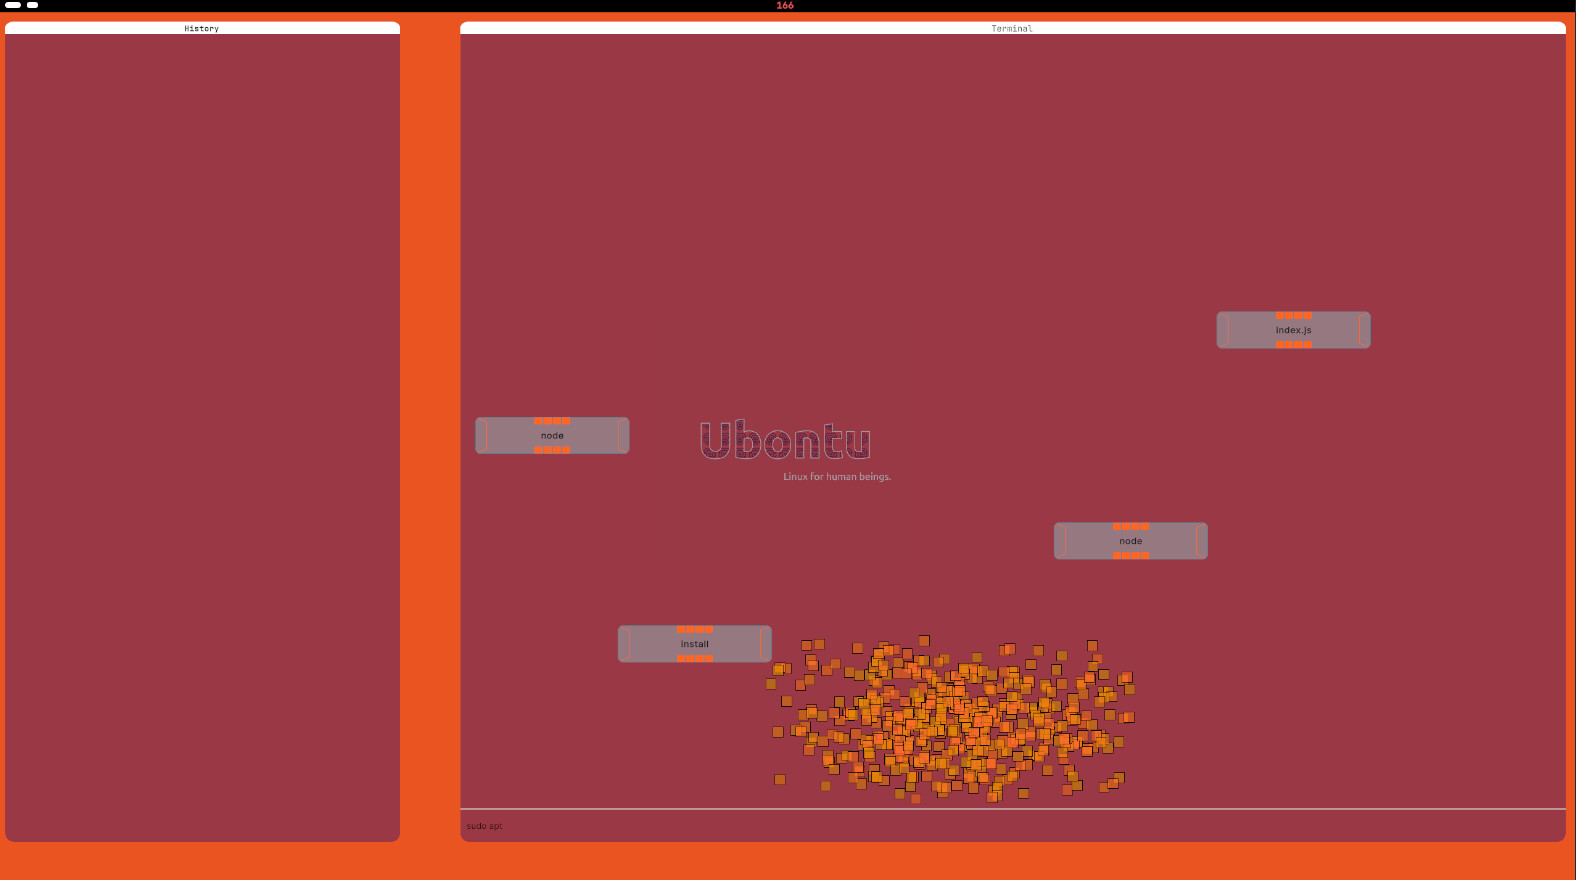
\includegraphics[width=0.65\textwidth]{images/MiniGameVFX.jpg}
    \caption{\ac{VFX} criado com o uso de \textit{frames} 2D criados com o \textit{framework} Processing.}
    \label{ProcessingVFX_WordRush}
\end{figure}

A Figura \ref{ProcessingVFX_WordRush} representa um caso prático onde os \textit{frames} criados com o \textit{framework} Processing foram utilizados para a construção de um efeito visual, quando o jogador acerta uma palavra no mini-jogo.

Além desse caso, na Figura \ref{ProcessingHomeMenu} é possível observar outro caso da utilização do Processing, onde foi utilizado para criar um conjunto de imagens 2D, as quais foram utilizadas para criar uma animação do menu principal do jogo, a qual é reproduzida quando o jogador inicia o jogo.

\begin{figure}[H]
    \centering
    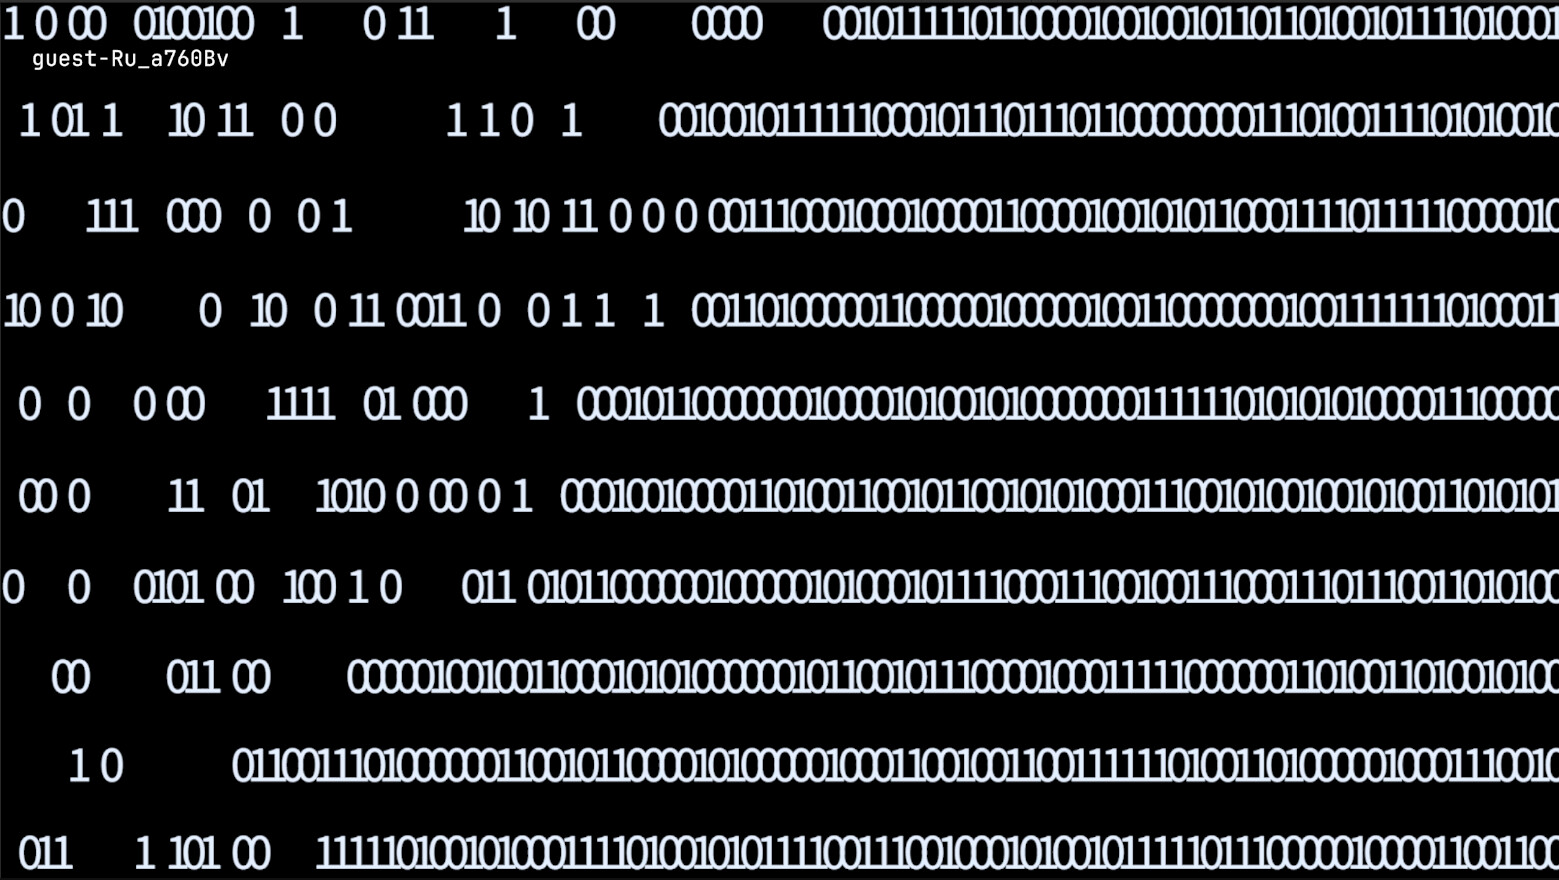
\includegraphics[width=0.65\textwidth]{images/HomeMenuEfeito.jpg}
    \caption{Animação do menu principal criada \textit{frame-by-frame} com a ajuda do \textit{framework} Processing.}
    \label{ProcessingHomeMenu}
\end{figure}

\subsection{Personagem}

\subsubsection{Modelo 3D}

\begin{figure}[H]
     \centering
     % Primeira Linha
     \begin{subfigure}[b]{0.3\textwidth}
         \centering
         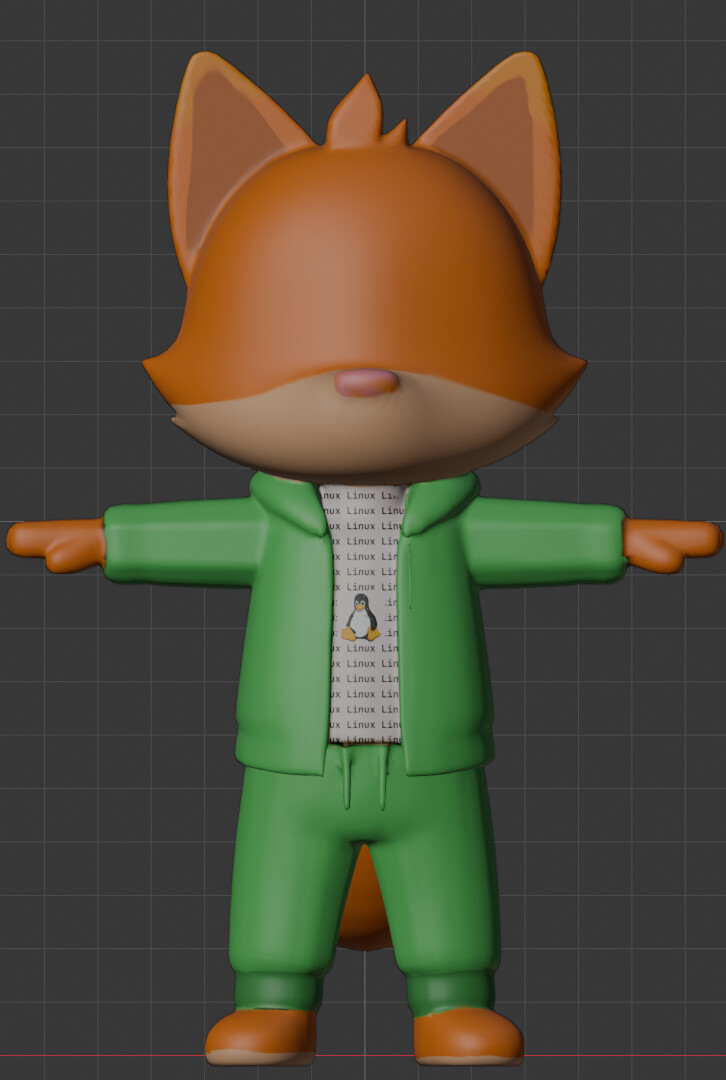
\includegraphics[width=\textwidth]{Presonagem/FurryFront.jpg}
     \end{subfigure}
     \hfill
     \begin{subfigure}[b]{0.3\textwidth}
         \centering
         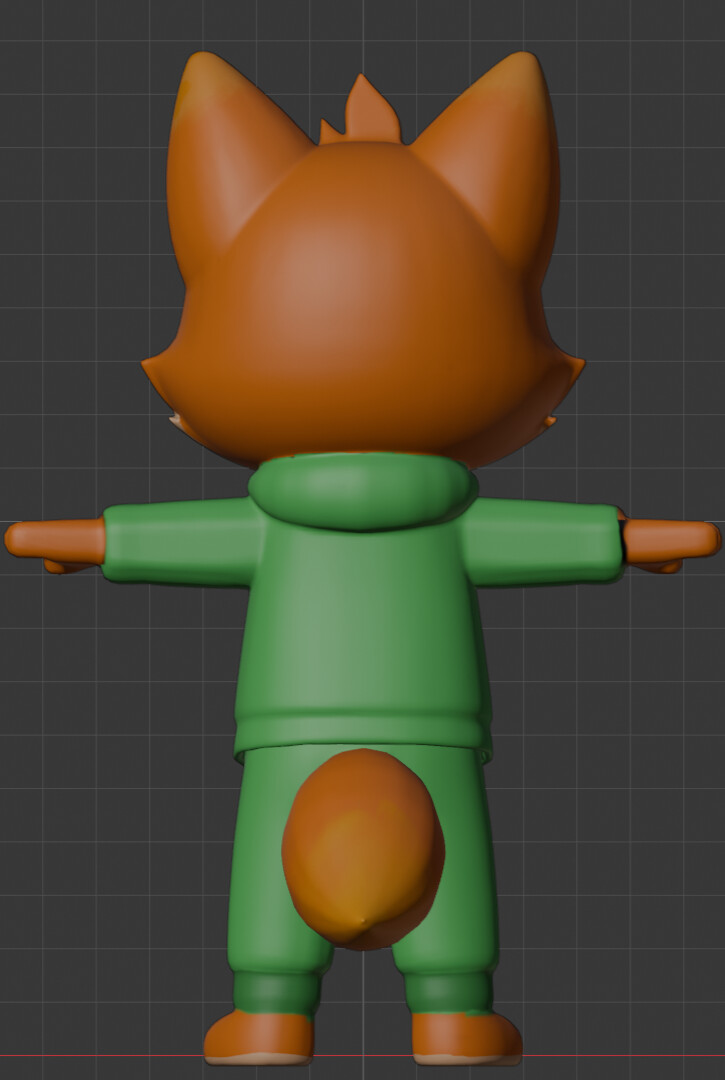
\includegraphics[width=\textwidth]{Presonagem/FurryBack.jpg}
     \end{subfigure}
     \hfill
     \begin{subfigure}[b]{0.3\textwidth}
         \centering
         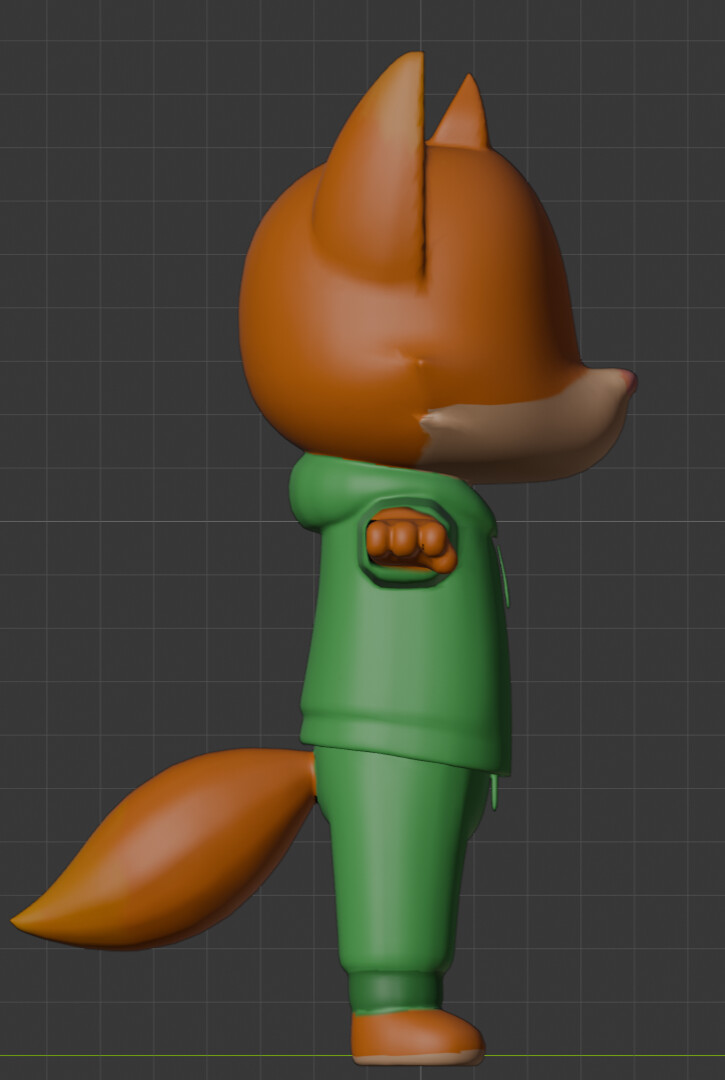
\includegraphics[width=\textwidth]{Presonagem/FurryLeft.jpg}
     \end{subfigure}

     \vspace{0.5cm} % Espaço entre as linhas

     % Segunda Linha
     \begin{subfigure}[b]{0.3\textwidth}
         \centering
         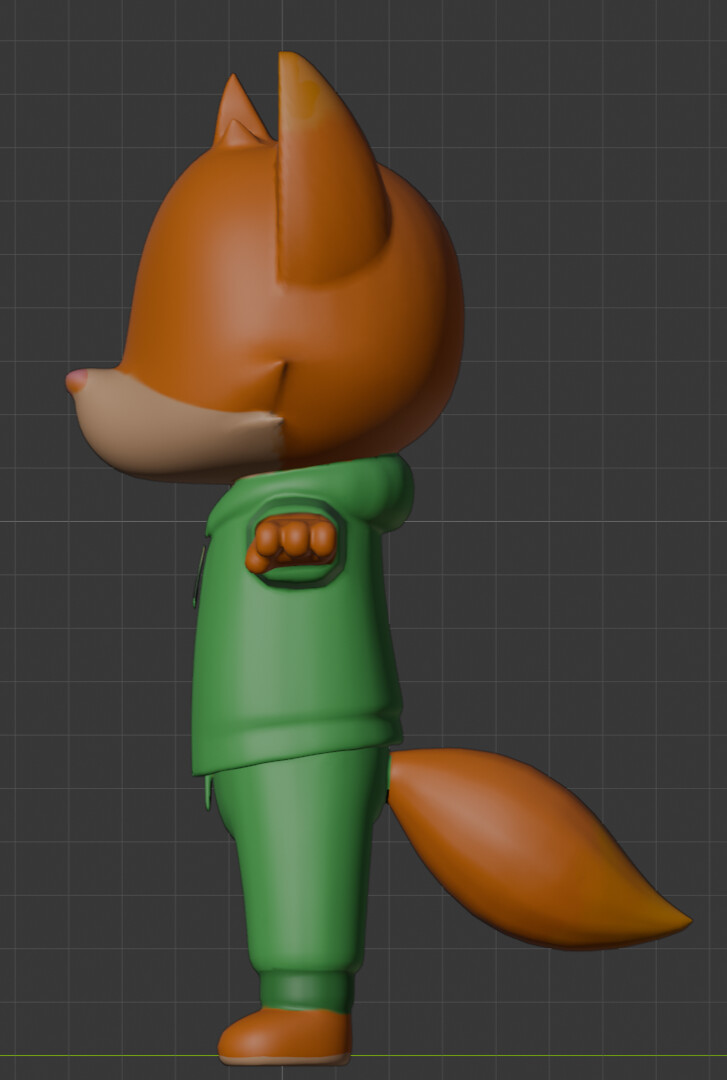
\includegraphics[width=\textwidth]{Presonagem/FurryRight.jpg}
     \end{subfigure}
     \hspace{0.5cm} % Espaço manual para centralizar a quinta imagem
     \begin{subfigure}[b]{0.3\textwidth}
         \centering
         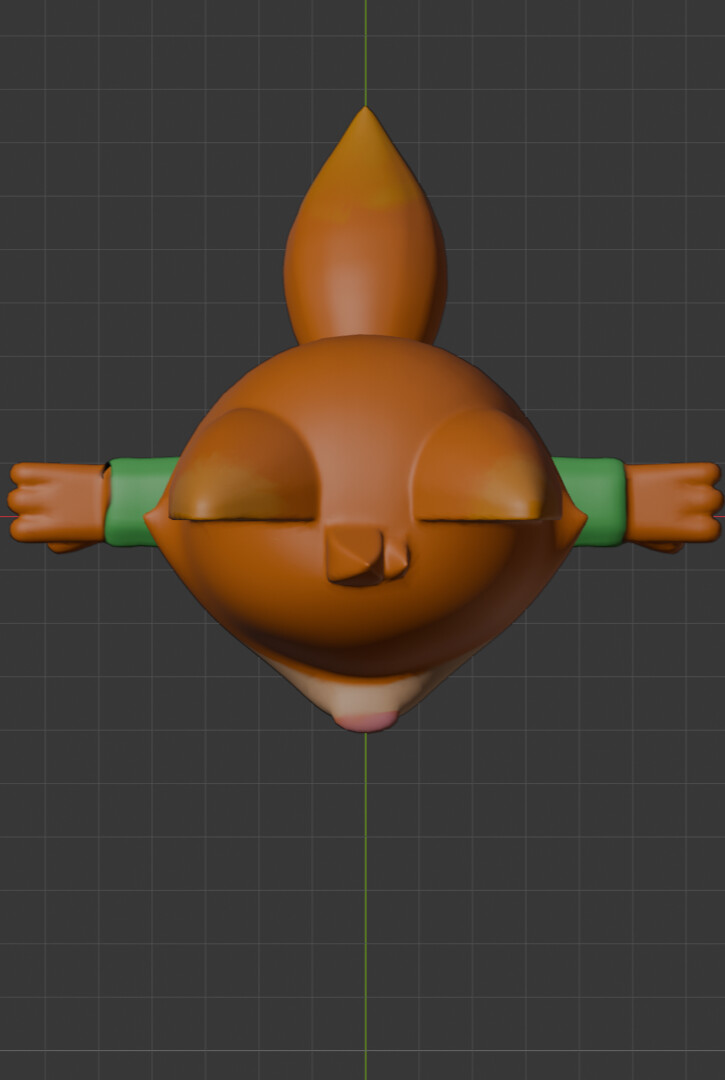
\includegraphics[width=\textwidth]{Presonagem/Furrytop.jpg}
     \end{subfigure}
     
     \caption{Modelo 3D do personagem, em várias vistas.}
     \label{characterManyLooks}
\end{figure}

O modelo 3D (\textit{mesh}) do personagem (Figura \ref{characterManyLooks}) foi criado com o auxílio da ferramenta de \ac{IA}, Chat 3D, usando como referência a Figura \ref{idealizacaoCharacter}. No entanto, a pintura de materiais e a construção de texturas, foram realizadas no \textit{software} Blender, utilizando o \textit{software} GIMP para desenvolver a textura da camisola branca.
O visual do personagem foi inspirado na mascote do \textbf{Mozilla Firefox}, uma vez que o jogo tem como tema central a internet, e o Firefox é um dos símbolos mais reconhecíveis da internet, o que faz com que seja uma fonte de inspiração bastante relevante para o projeto.

\subsubsection{Esqueleto e animações}

Um esqueleto de um modelo 3D é uma estrutura interna composta por um conjunto de “ossos” virtuais organizada de forma hierárquica, que serve para controlar a deformação e o movimento de um objeto tridimensional.

O esqueleto do modelo 3D é relevante, pois é através dele que é possível criar animações para o modelo, tais, como animações de caminhada, corrida, \textit{idel}, etc\dots.
O esqueleto do personagem foi criado no \textit{website} \textit{Mixamo}, onde também foram retidas as animações de caminhada, corrida e \textit{idle}. 

Após isso, o modelo 3D do personagem, com o esqueleto e as animações, foram importados para a Unity, onde foram feitos ajustes para que as animações pudessem ser reproduzidas de forma fluida e natural.

\subsection{Implementação do sistema de Ataque}
\label{Sec:ImplementSistemaAtaque}

\todo{Revisar}
O sistema de ataque é responsável por desencadear os ataques ao longo do jogo. Este sistema funciona de forma periódica e constante, sendo responsável pela criação dos ataques e pela instanciação dos inimigos no cenário.

Um novo ataque ocorre sempre que o jogador completa um determinado número de novas tarefas. Cada ataque encontra-se associado a um e-mail, que o jogador é obrigado a ler. O e-mail (ver Subsecção \ref{Sec:Email}) apresenta o ataque e o seu propósito, contribuindo para uma maior integração do mesmo no contexto do jogo. Para além disso, o e-mail pode também ser utilizado como meio para transmitir informação adicional ao jogador. O e-mail também atua como \textit{trigger} para a ação, enquanto o jogador não ler o e-mail o estado do jogo não se altera.

Durante o período de um ataque, o jogador pode utilizar o canhão (ver Subsecção \ref{Sec:Canhão}) presente no cenário. Para superar o ataque, o jogador terá de destruir todos os inimigos presentes no cenário.

\begin{figure}[H]
\centering
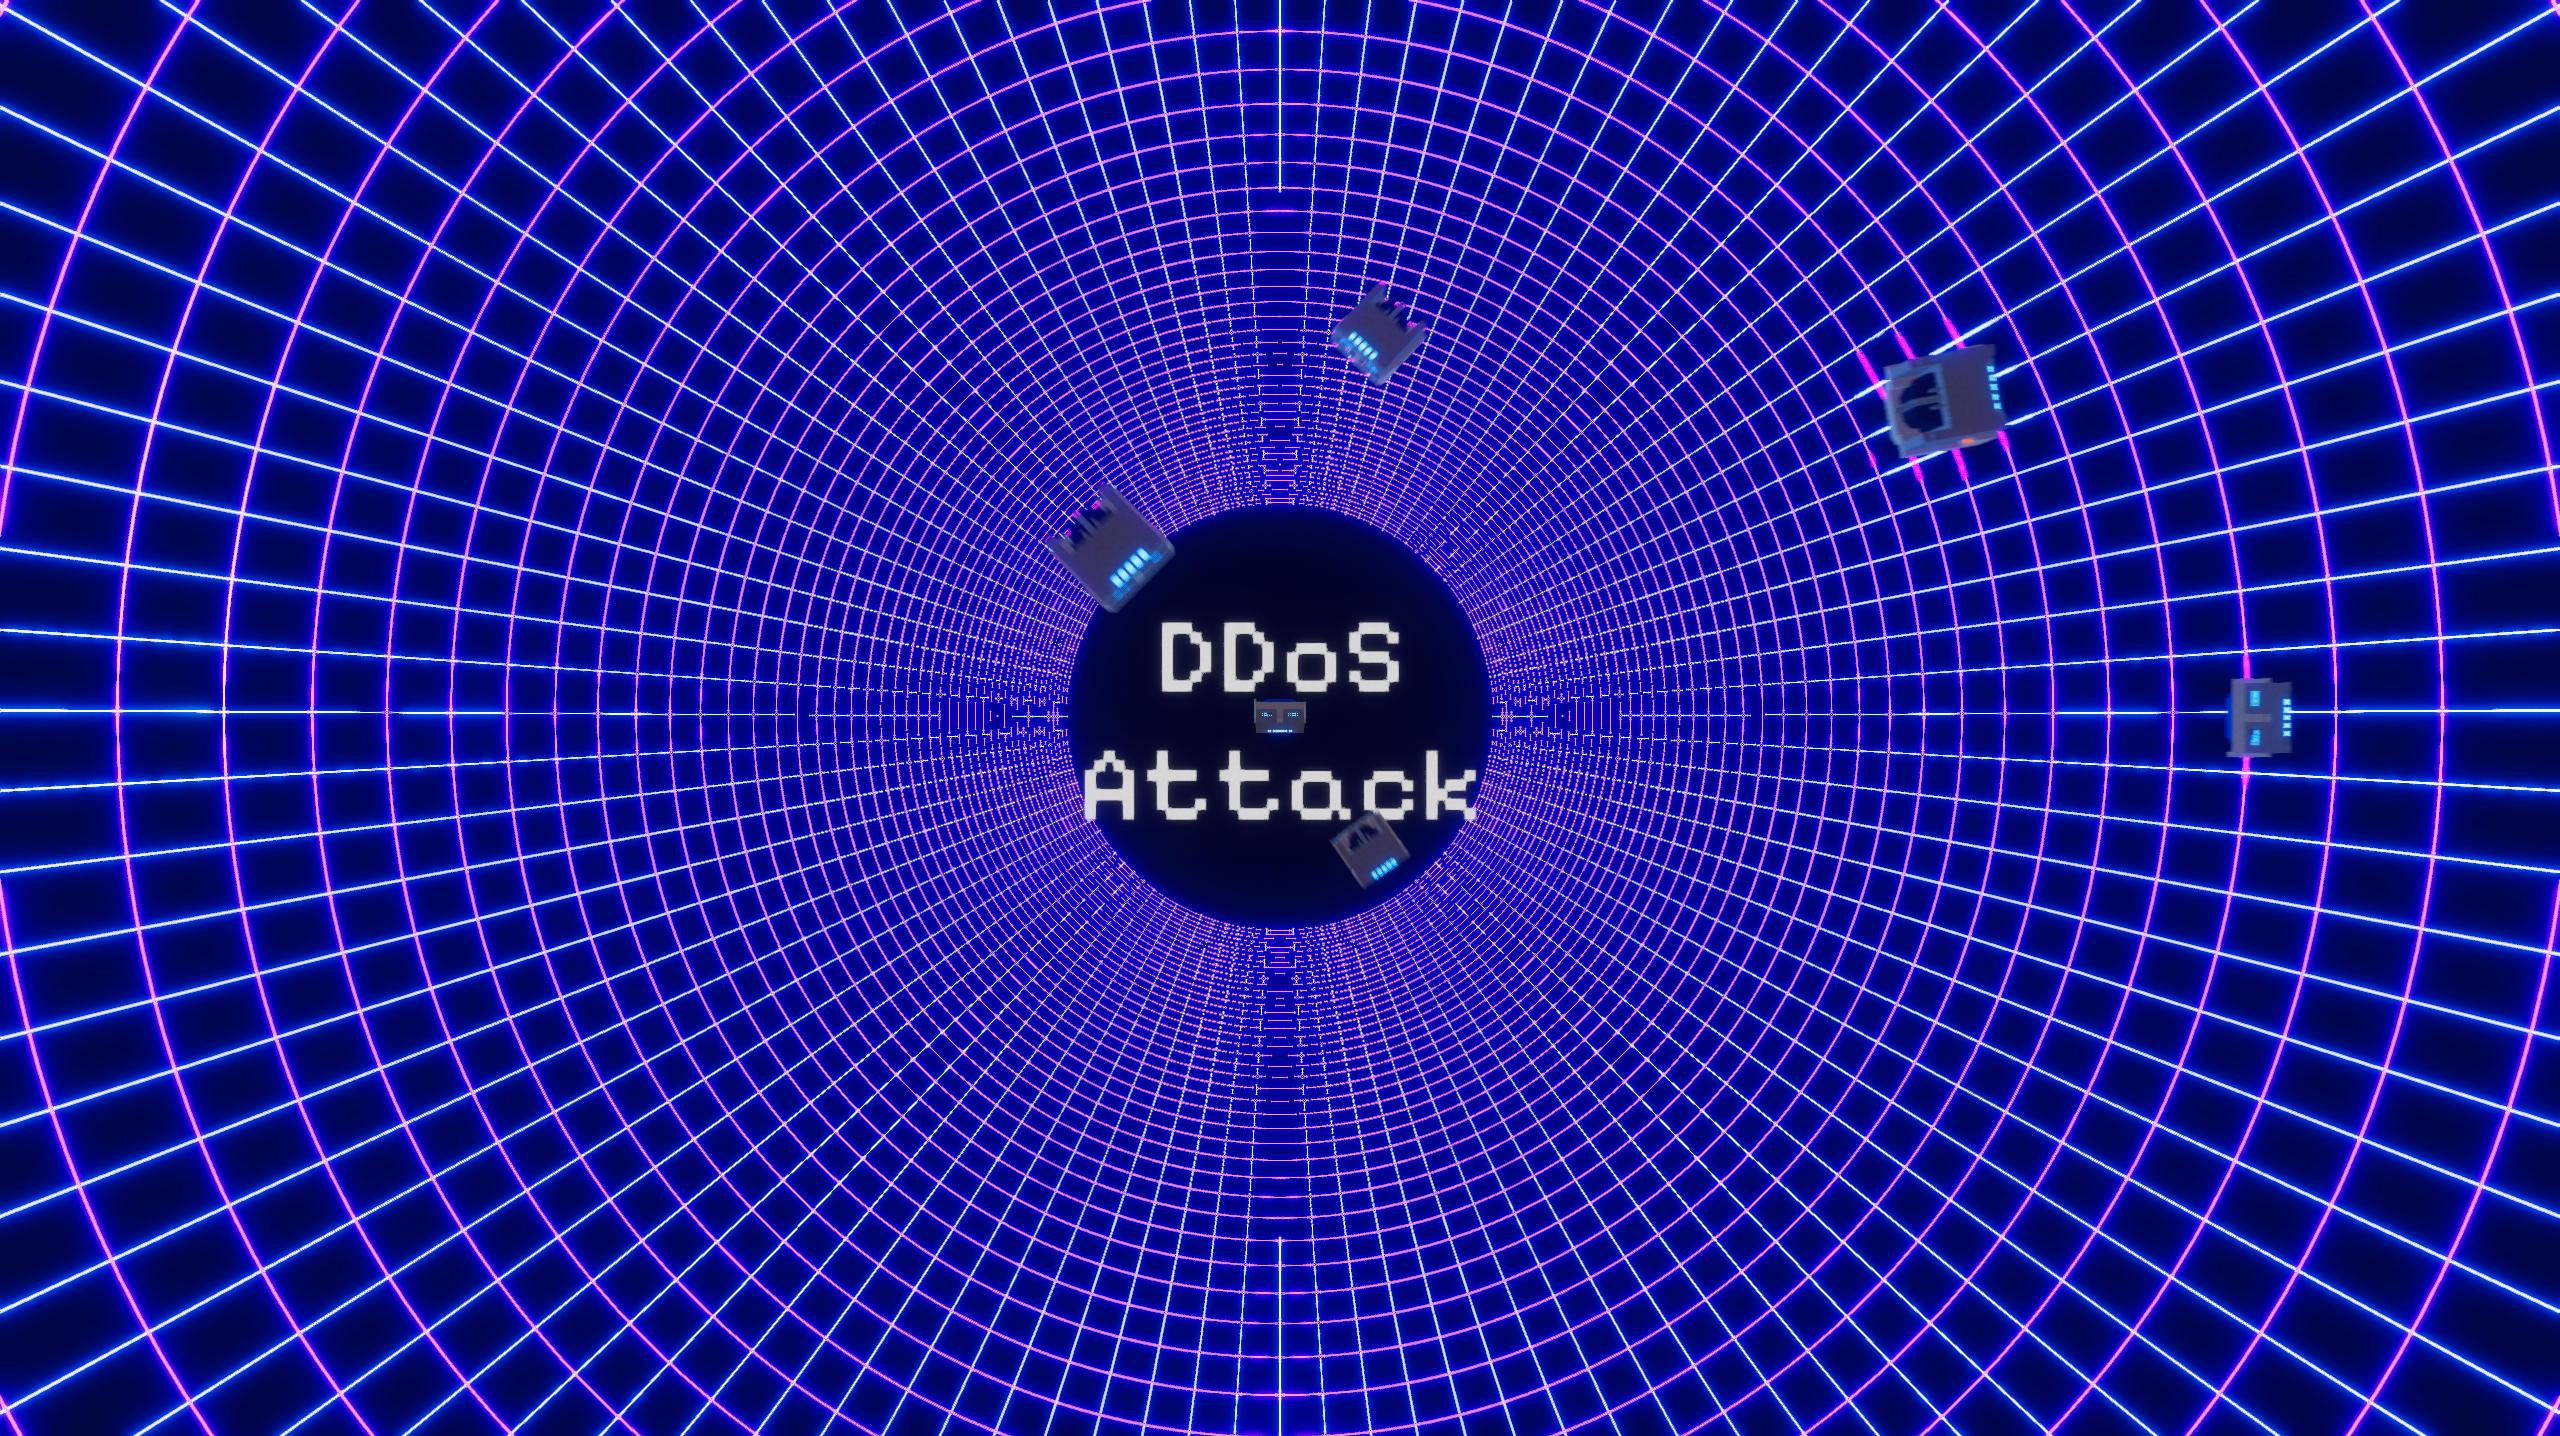
\includegraphics[width=0.65\textwidth]{images/Attack Launch.png}
\caption{Animação de início do ataque.}
\label{Launch Attack}
\end{figure}

\begin{figure}[H]
\centering
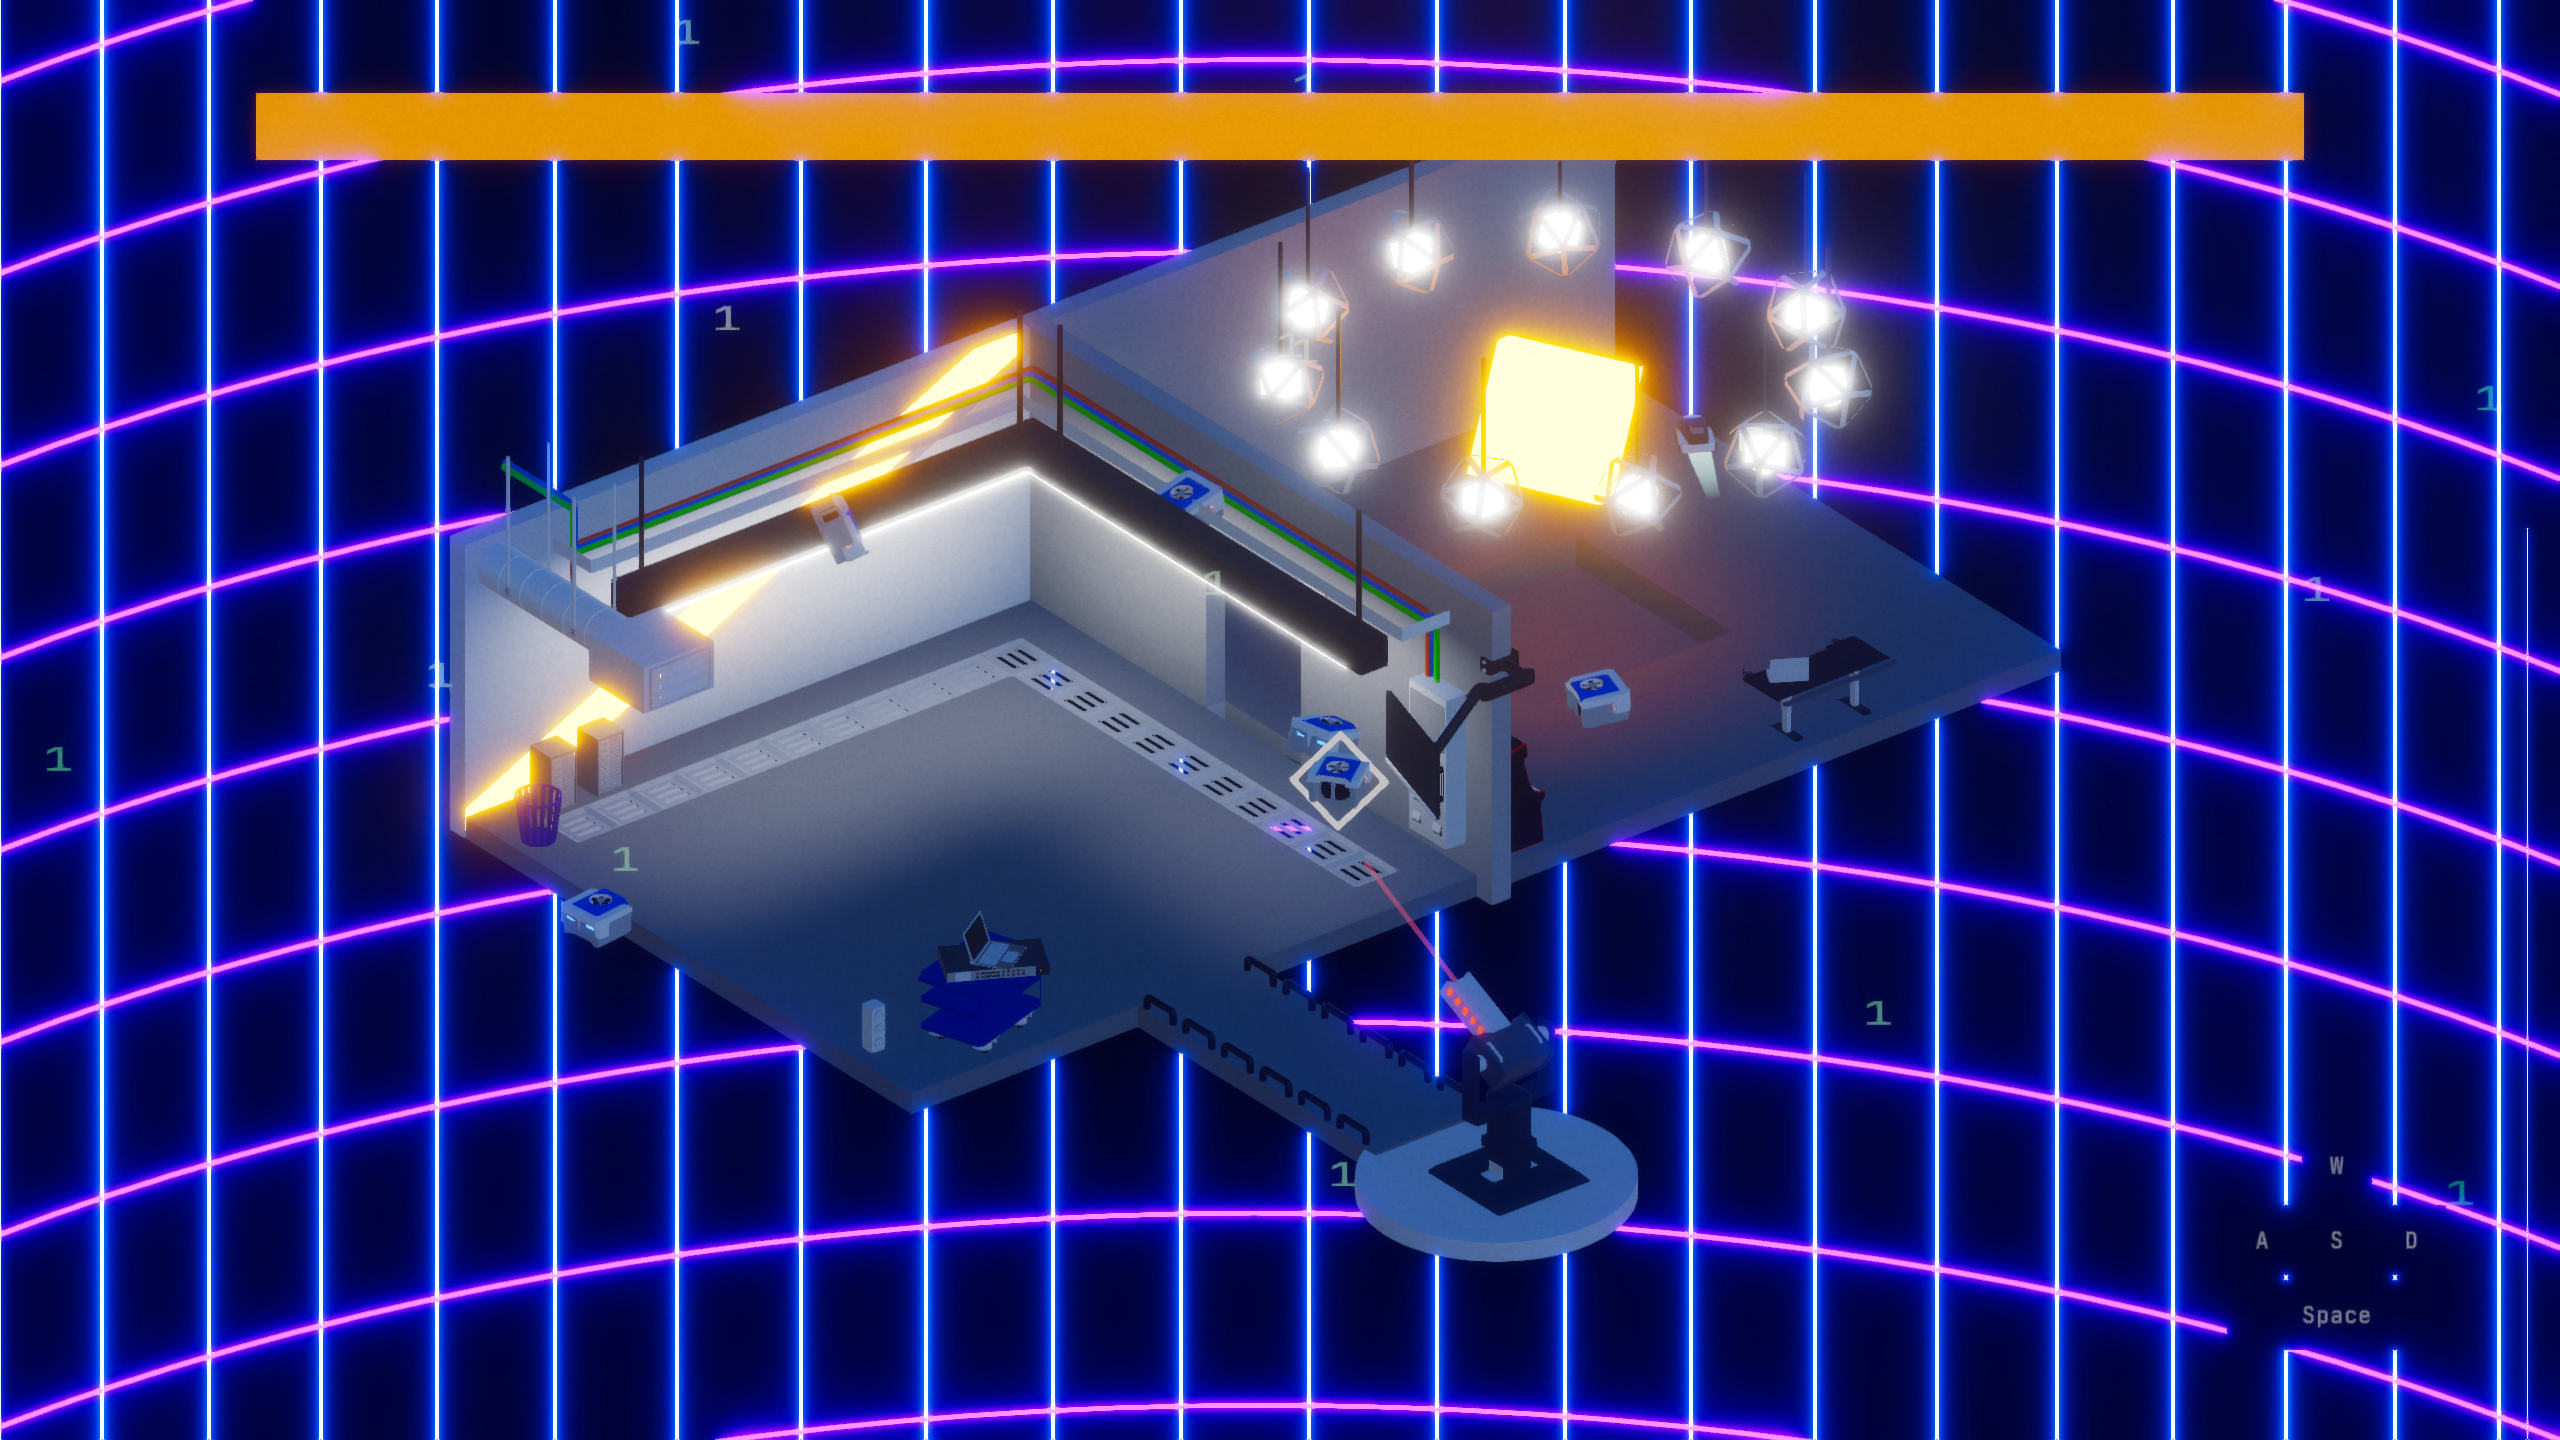
\includegraphics[width=0.65\textwidth]{images/Cannon Aim.png}
\caption{Mecânica de mira do canhão durante um ataque.}
\label{Cannon Aim}
\end{figure}

A Figura \ref{Launch Attack} representa a animação apresentada sempre que se inicia um novo ataque. A principal função desta animação é contextualizar o jogador relativamente ao ataque que se inicia, apresentando o seu nome e permitindo-lhe preparar-se para a invasão. Durante esta animação, o estado do mundo permanece inalterado, garantindo ao jogador um período de preparação antes do início do ataque.

A Figura \ref{Cannon Aim} representa a perspetiva do jogador durante um ataque. Neste contexto, o jogador deixa de controlar diretamente a personagem e passa a controlar o canhão presente no cenário. Na parte superior do ecrã encontra-se uma barra centralizada que representa a percentagem de inimigos que ainda permanecem no cenário. Assim, quanto menor for o valor apresentado, menor será o número de inimigos que falta destruir.

Uma vez que a câmara utilizada neste \textit{minijogo} é a mesma utilizada no restante jogo, sendo esta uma câmara ortográfica, não existe perspetiva nem perceção de profundidade através da escala dos objetos. Esta característica torna a tarefa de apontar mais difícil, pelo que foram implementados mecanismos adicionais para facilitar a mira. Na extremidade do canhão foi adicionado um laser que funciona como auxiliar de mira. Adicionalmente, quando a mira se encontra sobre um inimigo, é apresentado um indicador branco à sua volta, permitindo identificar de forma mais clara o alvo selecionado.

Estas funcionalidades foram implementadas com o objetivo de melhorar a experiência de mira do jogador, compensando a ausência de perspetiva e, consequentemente, a reduzida perceção de profundidade proporcionada pela câmara ortográfica.

Para compreender melhor a forma como o sistema de ataque interage com os restantes sistemas do jogo, podem ser consultadas as Subsecções \ref{Sec:DiagramaSistemaJogo} e \ref{Sec:Canhão}.


\todo{Até Aqui}

\subsection{Implementação do \textit{WordRush}}
\label{Sec:WordRush}

\todo{Revisar}
O \textit{WordRush} é o principal \textit{minigame} presente no projeto, uma vez que é responsável por simular a execução das tarefas. A sua utilização ocorre como consequência direta da aceitação de uma tarefa, que é comunicada ao jogador através de uma notificação (consultar a Secção \ref{Sec:Notify} para mais informações sobre o sistema de notificações).

O objetivo deste \textit{minigame} é simular um terminal no qual o jogador deve escrever um conjunto de palavras que surgem no ecrã e que, quando corretamente introduzidas, permitem a execução de comandos. Estes comandos estão diretamente relacionados com o tipo de tarefa previamente aceite pelo jogador. Em termos visuais, a interface foi inspirada no ambiente gráfico \textit{GNOME} (ver Subsecção \ref{Sec:ReferenciasReais}) e no jogo \textit{Grey Hack} (ver Subsecção \ref{Sec:GreyHack}).

Como pode ser observado na Figura \ref{WordRush Current}, a interface do \textit{WordRush} encontra-se dividida em três áreas principais. A área central direita corresponde à zona onde as palavras surgem e se deslocam pelo ecrã. Na zona inferior direita encontra-se o campo de introdução, onde o jogador escreve as palavras apresentadas. Por sua vez, a área lateral esquerda apresenta os comandos que foram introduzidos pelo jogador, acompanhados de uma breve descrição da função de cada um.

As palavras apresentadas ao jogador variam de acordo com o tipo de tarefa que está a ser executada, sendo igualmente atribuída uma pontuação (\textit{score}) distinta consoante as palavras ou comandos introduzidos. Desta forma, o \textit{WordRush} adapta a sua jogabilidade ao contexto da tarefa, permitindo representar diferentes tipos de atividades através de uma mesma mecânica de interação.

\begin{figure}[H]
\centering
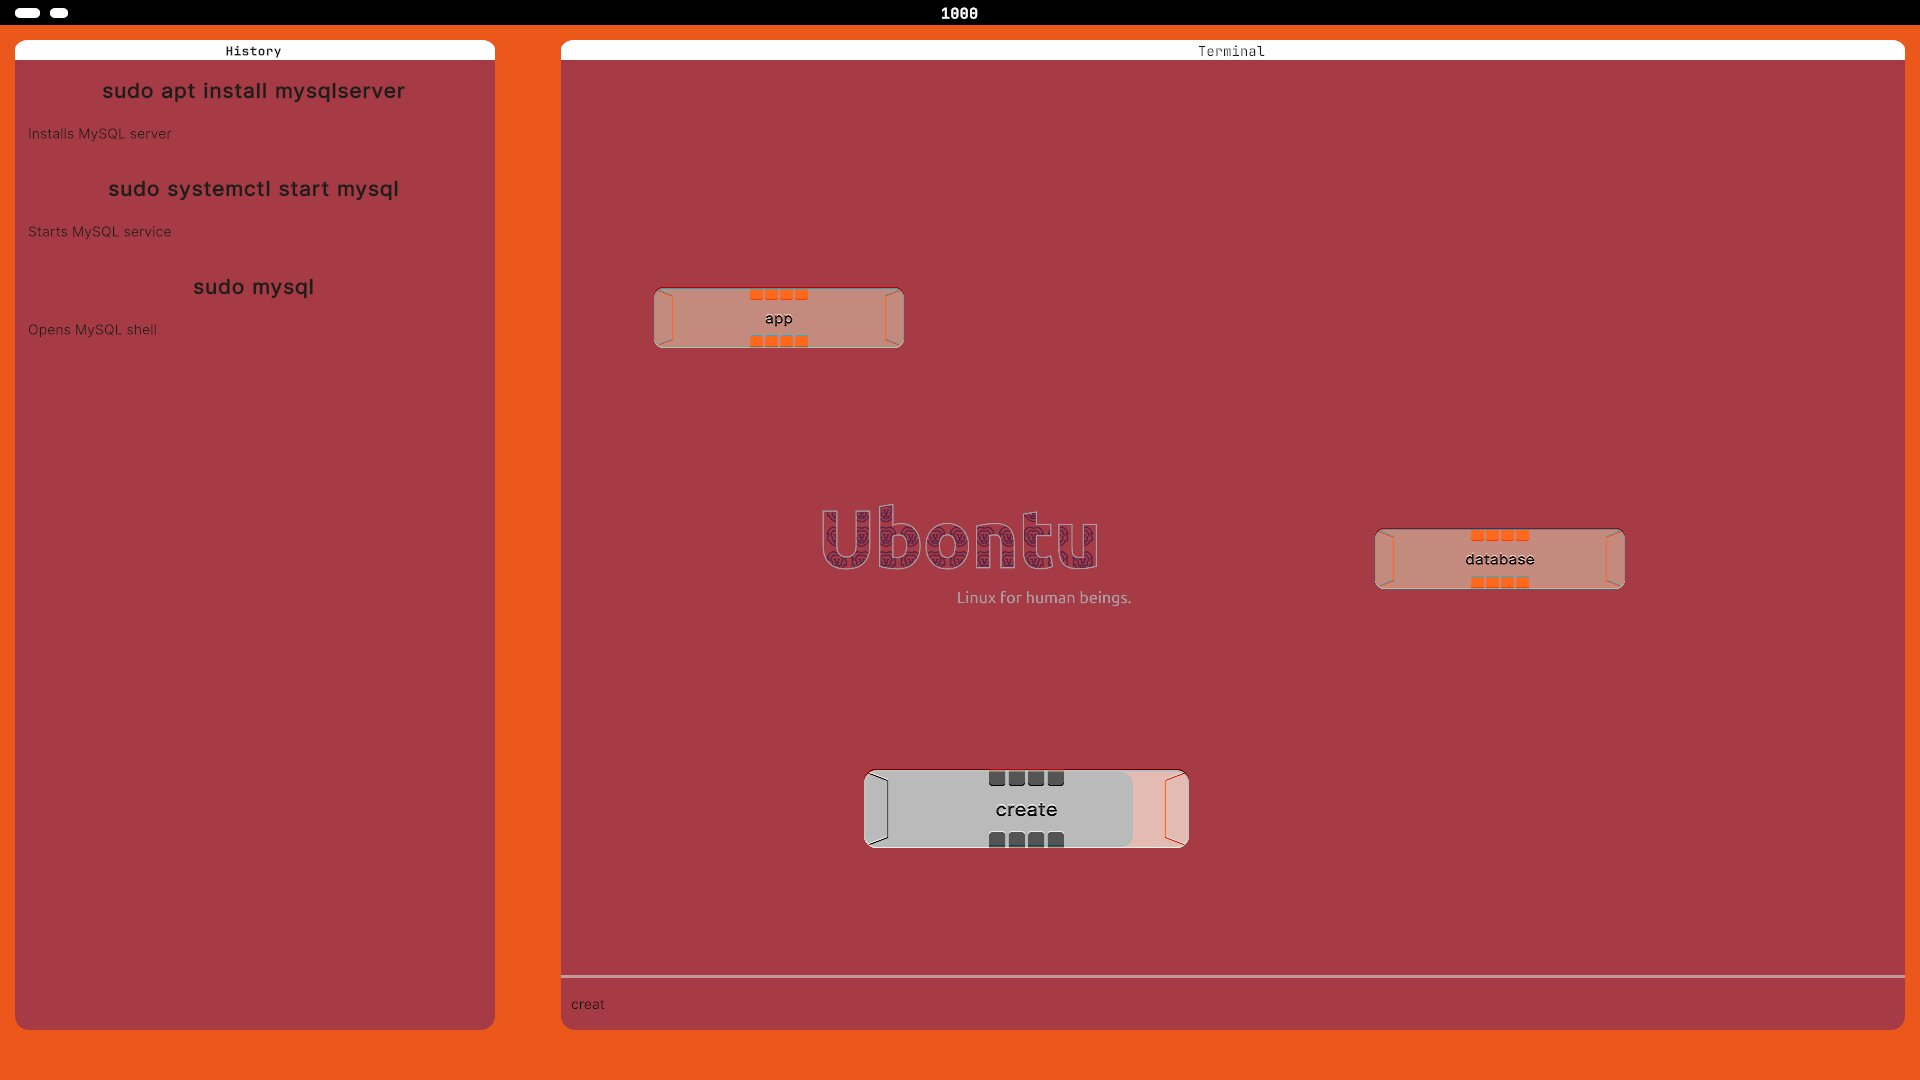
\includegraphics[width=0.65\textwidth]{images/WordRush.jpg}
\caption{\textit{Minigame WordRush}.}
\label{WordRush Current}
\end{figure}

\begin{figure}[H]
\centering
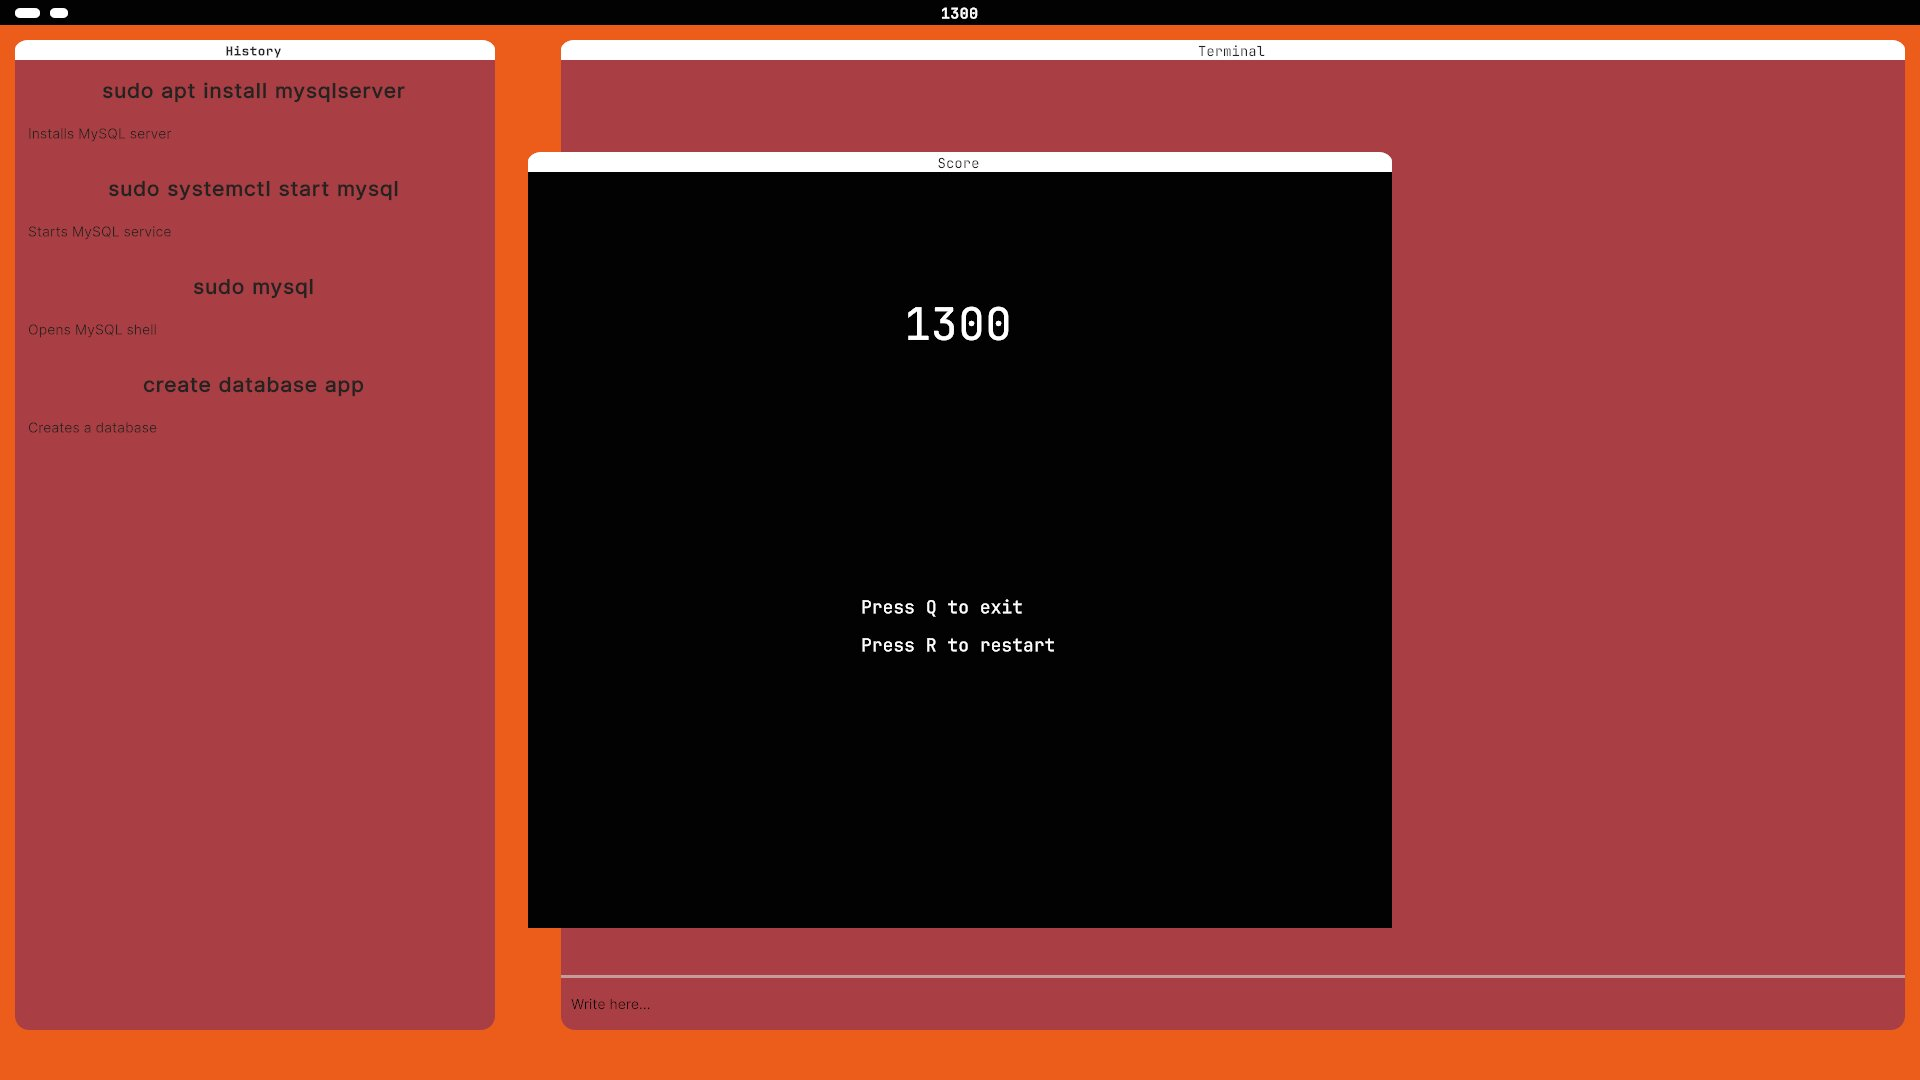
\includegraphics[width=0.65\textwidth]{images/WordRushFinished.jpg}
\caption{Tela final do \textit{minigame WordRush}.}
\label{WordRush Finished}
\end{figure}

\todo{Aqui}